



A large amount of physics (and indeed applied mathematics as a whole) is governed by a rather small collection of partial differential equations: the wave equation, the diffusion equation and Laplace's equation. The aim of this course is to build up a toolbox of techniques for solving these equations, and equations like them.
The tools themselves -- Fourier series, Sturm--Liouville theory, Green's functions, Fourier transforms and the method of characteristics -- are united by a single underlying idea, that of \emph{linearity}. Almost everything we do will amount to breaking a complicated problem into simple pieces (usually eigenfunctions or point sources), solving each piece, and adding up the results.

This article constitutes my notes for the `Methods' course, held in Michaelmas 2021 at Cambridge. These notes are \emph{not a transcription of the lectures}, and differ significantly in quite a few areas. Still, all lectured material should be covered.



\section{Fourier Series}

\subsection{Periodic Functions}

We will begin our study of methods and in particular Fourier series by considering some periodic functions.

\begin{definition}[Periodic]
    A function $f(x)$ is \vocab{periodic} if $f(x + T) = f(x)$ for all $x$, where $T$ is the \vocab{period}.
\end{definition}

\begin{example}[Simple Harmonic Motion]
    Many physical objects are described by \emph{simple harmonic motion}, with the position given by
    $$
    y = A \sin \omega t.
    $$
    We call $A$ the \vocab{amplitude}, and the period is $T = 2 \pi / \omega$. The \vocab{frequency} is $1/T$.
\end{example}

Fourier series is all about trying to write periodic functions as particular sums of sines and cosines.
Consider the set of functions
$$
g_n(x) = \cos \frac{n \pi x}{L}, \quad \text{and} \quad h_n(x) = \sin \frac{n \pi x}{L},
$$
where we take $n \in \N$.  These functions are periodic with period $2L$.

You may recall the following set of identities:
\begin{align*}
    \cos A \cos B &= \frac{1}{2}\left(\cos(A - B) + \cos(A + B)\right) \\
    \sin A \sin B &= \frac{1}{2}\left(\cos(A - B) - \cos(A + B)\right) \\
    \sin A \cos B &= \frac{1}{2}\left(\sin(A - B) + \sin(A + B)\right).
\end{align*}
We are going to try and define an inner product on this domain $[0, 2L]$, and using that we will by able to multiply these functions together and talk about their relative orthogonality.

\begin{definition}
    We define the inner product
    $\langle f, g \rangle = \int_0^{2L} f(x) g(x) \dd x$.
\end{definition}

We can then obtain some orthogonality conditions for $h_n$ and $g_n$ with respect to this inner product. We can compute for $n \neq m$
\begin{align*}
    \langle h_n, h_m \rangle &= \int_0^{2L} \sin \frac{n \pi x}{L} \sin \frac{m \pi x}{L} \dd x \\
    &= \frac{1}{2}\int_0^{2L} \left(\cos \frac{(n -m) \pi }{L}x - \cos \frac{(n + m )\pi}{L} x\right) \dd x \\
    &= \frac{1}{2} \frac{L}{\pi}\left[\frac{\sin (n - m) \pi x /L}{n - m} - \frac{\sin (n + m) \pi x /L}{n + m}\right]_0^{2L} \\
    &= 0,
\end{align*}
and for $n = m$
\begin{align*}
    \langle h_n, h_n \rangle &= \int_0^{2L} \sin^2 \frac{n \pi x}{L} \dd x \\
                             &= \int_0^{2L} \frac{1}{2}\left(1 - \cos \frac{2 \pi n x}{L}\right) \dd x \\
                             &= L.
\end{align*}
Hence we obtain the orthogonality condition
$$
\langle h_n, h_m \rangle = \begin{cases}
    L \delta_{mn} &\mbox{if } n, m \neq 0, \\
    0 &\mbox{if } m = 0.
   \end{cases}
$$
Similarly, it's straightforward to check that
$$
\langle g_n, g_m \rangle = \begin{cases}
    L \delta_{mn} &\mbox{if } n, m \neq 0, \\
    2L \delta_{0n} &\mbox{if } m = 0.
   \end{cases}
$$
and
$$
\langle h_n, g_m \rangle = 0.
$$

These orthogonality conditions are important because we are going to use these functions as a complete orthogonal set which spans the space of `well-behaved periodic functions'.


\subsection{Definition of a Fourier Series}

We can express any `well-behaved' periodic function $f(x)$ with period $2L$ as
$$
f(x)=\frac{1}{2} a_{0}+\sum_{n=1}^{\infty} a_{n} \cos \frac{n \pi x}{L}+\sum_{n=1}^{\infty} b_{n} \sin \frac{n \pi x}{L},
$$
where $a_n$, $b_n$ are constants such that the RHS is convergent for all $x$ where $f$ is continuous. At a discontinuity, the Fourier series approaches the midpoint of the upper and lower limits at that point.

Consider taking the inner product $\langle h_m, f\rangle$ and substitute the expression for $f$ above, to get
$$
   \int_0^{2L} \sin \frac{m\pi x}{L} f(x) \dd x = \sum_{n = 1}^{\infty} L b_n \delta_{nm} = Lb_m.
$$
Hence we find that (doing something similar with $g_n$)
\begin{align*}
   b_n &= \frac{1}{L}\int_0^{2L} f(x) \sin \frac{n \pi x}{L} \dd x, \\
    \text{and} \quad a_n &= \frac{1}{L}\int_0^{2L} f(x) \cos \frac{n \pi x}{L} \dd x.
\end{align*}

Now, this expression for $a_n$ includes the case $n = 0$, and says that $\frac{1}{2}a_0$ is the average value of the function. Also, the range of integration is one period, and we can equivalently integrate over $[-L, L]$ instead of $[0, 2L]$.

\begin{example}[The Sawtooth Wave]
    Consider the function $f(x) = x$ for $-L \leq x \leq L$, with the function being periodic elsewhere.


	\begin{center}
		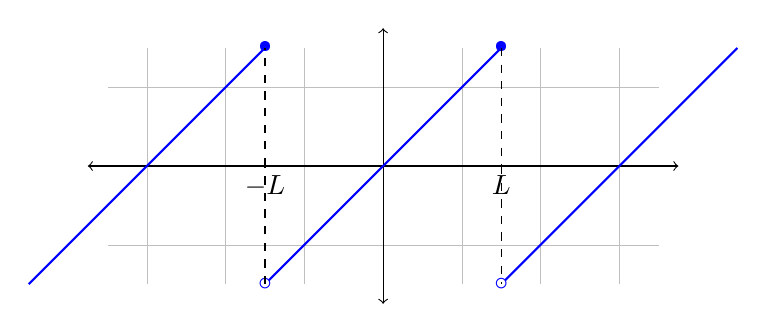
\begin{tikzpicture}
	  \draw[ultra thin,color=lightgray] (-3.5,-1.5) grid (3.5,1.5);   % coordinate grid
	  \draw[<->] (-3.75,0) -- (3.75,0);% node[right] {$x$};   % x-axis
	  \draw[<->] (0,-1.75) -- (0,1.75);% node[above] {$y$};   % y-axis

      \draw [thick, samples=100,smooth, color=blue] plot[variable=\t, domain=-4.5:-1.5] ({\t},{\t + 3});
      \draw [thick, samples=100,smooth, color=blue] plot[variable=\t, domain=-1.45:1.5] ({\t},{\t});
      \draw [thick, samples=100,smooth, color=blue] plot[variable=\t, domain=1.55:4.5] ({\t},{\t - 3});

      \node at (-1.5, -1.5) {\color{blue} $\circ$};
	\node at (-1.5, 1.5) {\color{blue} \textbullet};

      \node at (1.5, -1.5) {\color{blue} $\circ$};
	\node at (1.5, 1.5) {\color{blue} \textbullet};

    \draw  [dashed] (1.5, 1.5) -- (1.5, 0) node [below] {$L$};
    \draw [dashed] (1.5, 0) -- (1.5, -1.5);
    \draw  [dashed] (-1.5, -1.5) -- (-1.5, 0) node [below] {$-L$};
    \draw [dashed] (-1.5, 0) -- (-1.5, 1.5);

	\end{tikzpicture}
	\end{center}

    Here we have
    $$
a_n = \frac{1}{L}\int_{-L}^L x \cos \frac{n \pi x}{L} \dd x = 0, \quad \quad \text{(integrating an odd function)}
    $$
    for all $n$, and
    \begin{align*}
        b_n &= \frac{2}{L} \int_0^L x \sin \frac{n \pi x}{L} \dd x   \\
            &= \frac{-2}{n \pi}\left[x \cos \frac{n \pi x}{L}\right]_{0}^{L} + \frac{2}{n \pi} \int_{0}^{L} \cos \frac{n \pi x}{L} \dd x \\
            &= -\frac{2 L}{n \pi} \cos n \pi+\frac{2 L}{(n \pi)^{2}} \cancel{\sin n \pi} \\
            &= \frac{2L}{n \pi} (-1)^{n + 1}.
    \end{align*}
    So the sawtooth Fourier series is
    $$
    2 L \sum_{n=1}^{\infty} \frac{(-1)^{n+1}}{n \pi} \sin \left(\frac{n \pi x}{L}\right)=\frac{2 L}{\pi}\left[\sin \left(\frac{\pi x}{L}\right)-\frac{1}{2} \sin \left(\frac{2 \pi x}{L}\right)+\frac{1}{3} \sin \left(\frac{3 \pi x}{L}\right) + \cdots\right].
    $$
    which is slowly convergent.

    %L = 1.5
    \begin{center}
    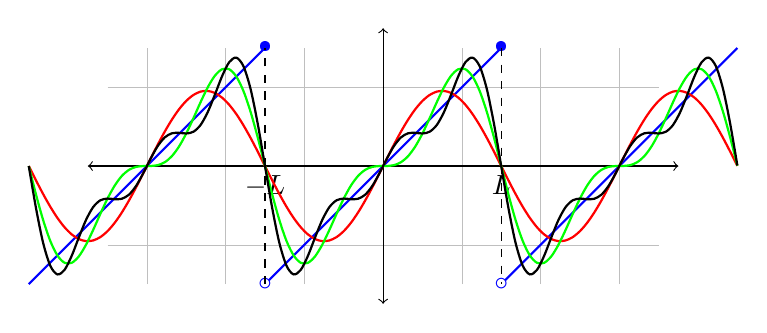
\begin{tikzpicture}
        \draw[ultra thin,color=lightgray] (-3.5,-1.5) grid (3.5,1.5);   % coordinate grid
        \draw[<->] (-3.75,0) -- (3.75,0);% node[right] {$x$};   % x-axis
        \draw[<->] (0,-1.75) -- (0,1.75);% node[above] {$y$};   % y-axis

        \draw [thick, samples=100,smooth, color=blue] plot[variable=\t, domain=-4.5:-1.5] ({\t},{\t + 3});
        \draw [thick, samples=100,smooth, color=blue] plot[variable=\t, domain=-1.45:1.5] ({\t},{\t});
        \draw [thick, samples=100,smooth, color=blue] plot[variable=\t, domain=1.55:4.5] ({\t},{\t - 3});

        \node at (-1.5, -1.5) {\color{blue} $\circ$};
      \node at (-1.5, 1.5) {\color{blue} \textbullet};

        \node at (1.5, -1.5) {\color{blue} $\circ$};
      \node at (1.5, 1.5) {\color{blue} \textbullet};

      \draw  [dashed] (1.5, 1.5) -- (1.5, 0) node [below] {$L$};
      \draw [dashed] (1.5, 0) -- (1.5, -1.5);
      \draw  [dashed] (-1.5, -1.5) -- (-1.5, 0) node [below] {$-L$};
      \draw [dashed] (-1.5, 0) -- (-1.5, 1.5);

      % Fourier Series

      \draw [thick, samples=100,smooth, color=red] plot[variable=\t, domain=-4.5:4.5] ({\t},{(2*1.5/pi) * (sin(180 * \t / 1.5))});
      \draw [thick, samples=100,smooth, color=green] plot[variable=\t, domain=-4.5:4.5] ({\t},{(2*1.5/pi) * (sin(180 * \t / 1.5) - 0.5 * sin(2 * 180 * \t / 1.5))});
      \draw [thick, samples=100,smooth, color=black] plot[variable=\t, domain=-4.5:4.5] ({\t},{(2*1.5/pi) * (sin(180 * \t / 1.5) - 0.5 * sin(2 * 180 * \t / 1.5) + (1/3) * sin(3 * 180 * \t / 1.5))});

      \end{tikzpicture}
      \end{center}
\end{example}

\subsection{The Dirichlet Conditions (Fourier's Theorem)}

So we need `well behaved' functions for what we have discussed about Fourier series to work, and for a Fourier series for $f$ to be unique. But what exactly does it mean for a function to be `well behaved' in this context?
This is specified by the Dirichlet conditions, also known as Fourier's theorem.

\begin{theorem}[The Dirichlet Conditions]
    If $f$ is a bounded periodic function with period $2L$ and finitely many minima, maxima and discontinuities on $0 \leq x \leq 2L$, then the Fourier series converges to $f(x)$ at all points where $f$ is continuous, and at discontinuities converges to $\frac{1}{2}(f(x_+) + f(x_-))$.
\end{theorem}

One might note that these conditions are \emph{much weaker} than those needed for Taylor series, but it does eliminate pathological functions such as $\sin 1/x$, $1/x$ and the indicator function on the rationals.
The converse of this is \emph{not} true, for example $\sin 1/x$ has a well defined Fourier series.

The proof of this result is \emph{too} difficult, but is best done using complex methods so we will not dwell on it in this course.

The rate of convergence of the Fourier series depends on the `smoothness' of the function.

\begin{theorem}[Rate of Convergence of Fourier Series]
If $f(x)$ has continuous derivatives up to a $p$th derivative which is discontinuous, then the Fourier series converges as $\mathcal{O}(n^{-(p + 1)})$ as $n \rightarrow \infty$.
\end{theorem}

\begin{example}[Square Wave]\label{ex:square}
    Consider the function
    $$
    f(x) = \begin{cases}
        1 &\mbox{if } 0 \leq x < 1, \\
        -1 &\mbox{if } -1 \leq x < 0.
       \end{cases}
    $$
    This function has discontinuous $p = 0$th derivative (the function is discontinuous!), and the Fourier series of this function is given by
    $$
    f(x) = 4 \sum_{m=1}^{\infty} \frac{\sin (2 m-1) \pi x}{(2 m-1) \pi}.
    $$
\end{example}

It is worth pausing to look at how the partial sums of this series actually behave. Below is the square wave along with the partial sums taking $m \leq 2$ and $m \leq 8$.

\begin{center}
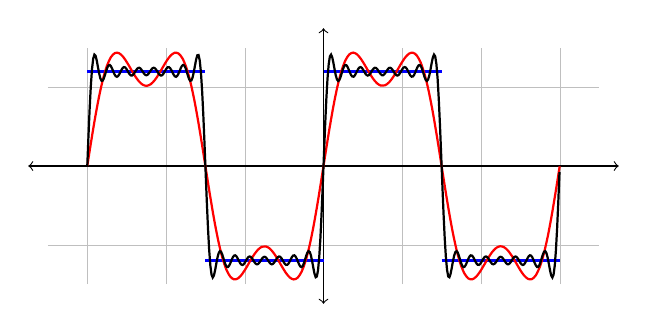
\begin{tikzpicture}
    \draw[ultra thin,color=lightgray] (-3.5,-1.5) grid (3.5,1.5);   % coordinate grid
    \draw[<->] (-3.75,0) -- (3.75,0);
    \draw[<->] (0,-1.75) -- (0,1.75);

    % square wave, L = 1, amplitude 1.2 (x-scale 1.5)
    \draw [thick, color=blue] (-3,1.2) -- (-1.5,1.2);
    \draw [thick, color=blue] (-1.5,-1.2) -- (0,-1.2);
    \draw [thick, color=blue] (0,1.2) -- (1.5,1.2);
    \draw [thick, color=blue] (1.5,-1.2) -- (3,-1.2);

    % partial sums (plot x in [-3,3], actual variable x = t/1.5)
    \draw [thick, samples=120,smooth, color=red] plot[variable=\t, domain=-3:3]
      ({\t},{1.2*(4/pi)*(sin(120*\t) + sin(3*120*\t)/3)});
    \draw [thick, samples=400, color=black] plot[variable=\t, domain=-3:3]
      ({\t},{1.2*(4/pi)*(sin(120*\t) + sin(3*120*\t)/3 + sin(5*120*\t)/5 + sin(7*120*\t)/7 + sin(9*120*\t)/9 + sin(11*120*\t)/11 + sin(13*120*\t)/13 + sin(15*120*\t)/15)});
\end{tikzpicture}
\end{center}

Away from the discontinuities the partial sums settle down quite quickly, but near each jump they consistently \emph{overshoot} by roughly $9\%$ of the size of the jump, and this overshoot does not go away as we take more terms -- it just gets squeezed into a narrower and narrower region around the discontinuity. This is the \vocab{Gibbs phenomenon}. It doesn't contradict the Dirichlet conditions (at each \emph{fixed} $x$ the series still converges), but it does tell us that the convergence is not uniform near a jump.

\subsubsection*{Integration of Fourier Series}

As a general principle, it is \emph{always} valid to integrate the Fourier series of $f(x)$ term-wise to obtain
$$
F(x) = \int_{-L}^x f(u) \dd u,
$$
because $F(x)$ satisfies the Dirichlet conditions if $f(x)$ does.

\subsubsection*{Differentiation of Fourier Series}

As a general principle, you must \emph{take care} when differentiating a Fourier series term-wise. Let's look at an example.

\begin{example}[Differentiating the Square Wave]
    Consider the clearly non-differentiable square wave function, defined in \autoref{ex:square}. We had
    $$
    f(x)=4 \sum_{m=1}^{\infty} \frac{\sin (2 m-1) \pi x}{(2 m-1) \pi}.
    $$
    We can try and differentiate this term-wise to get
    $$
    f^{\prime}(x) \stackrel{?}{=} 4 \sum_{m=1}^{\infty} \cos (2 m-1) \pi x,
    $$
    but this series is unbounded!
\end{example}

So we need to be careful. Here's the result about what we can do with differentiation.

\begin{theorem}
    If $f(x)$ is continuous and satisfies the Dirichlet conditions, and $f'(x)$ satisfies the Dirichlet conditions, then $f'(x)$ can be found by term-wise differentiation of the Fourier series of $f(x)$.
\end{theorem}

\subsection{Parseval's Theorem}

Parseval's theorem is a relation between the integral of the square of a function and the square of the Fourier coefficients:

\begin{align*}
    \int_{0}^{2L}[f(x)]^{2} \dd x&=\int_{0}^{2 L} \dd x\left[\frac{1}{2} a_{0}+\sum_{n} a_{n} \cos \frac{n \pi x}{L}+\sum_{n} b_{n} \sin \frac{n \pi x}{L}\right]^{2} \\
&= \int_{0}^{2 L} \dd x\left[\frac{1}{4} a_{0}^{2}+\sum_{n} a_{n}^{2} \cos ^{2} \frac{n \pi x}{L}+\sum_{n} b_{n}^{2} \sin ^{2} \frac{n \pi x}{L}\right] \\
&= L\left[\frac{1}{2} a_{0}^{2}+\sum_{n=1}^{\infty}\left(a_{n}^{2}+b_{n}^{2}\right)\right],
\end{align*}
where the cross terms all vanish by orthogonality.

This result is also called the completeness relation, since the LHS $\geq$ RHS if any of the basis functions are missing.

\begin{example}[The Basel Problem]
    Consider the sawtooth wave $f(x) = x$ on $-L \leq x \leq L$. Then the LHS is
    $$
    \int_{-L}^{L} x^2 \dd x = \frac{2}{3}L^3,
    $$
    and the RHS is
    $$
    L \sum_{n = 1}^{\infty} \frac{4L^2}{n^2 \pi^2} = \frac{4L^3}{\pi^2}\sum_{n = 1}^{\infty} \frac{1}{n^2},
    $$
    and thus $\sum_{n = 1}^{\infty} 1/n^2 = \pi^2/6$.
\end{example}


\subsection{Alternative Fourier Series}

There are some alternative forms of Fourier series.

\subsubsection*{Half-Range Series}

Consider $f(x)$ defined only on $0 \leq x < L$. We can extend its range over $-L \leq x < L$ in two simple ways:
\begin{enumerate}
    \item Require $f$ to be odd, with $f(-x) = -f(x)$. Then considering its Fourier series we would have $a_n = 0$ for all $n$ (as $\cos$ is even), and
    $$
    b_{n}=\frac{2}{L} \int_{0}^{L} f(x) \sin \frac{n \pi x}{L} \dd x.
    $$
    This implies that $f(x) = \sum_{n= 1}^{\infty} b_n \sin \frac{n \pi x}{L}$, which is a \vocab{Fourier sine series}.
    \item Require $f$ to be even, with $f(-x) = f(x)$, Then $b_n = 0$, and
    $$
    a_{n}=\frac{2}{L} \int_{0}^{L} f(x) \cos \frac{n \pi x}{L} \dd x,
    $$
    so $f(x) = \frac{1}{2}a_0 + \sum_{n = 1}^{\infty} a_n \cos\frac{n \pi x}{L}$, which is a \vocab{Fourier cosine series}.
\end{enumerate}

\subsubsection*{Complex Representation}

Recall that we can write
$$
\cos \frac{n \pi x}{L} = \frac{1}{2}\left(e^{in \pi x/L} + e^{-i n \pi x/L}\right) \quad \text{and} \quad \sin \frac{n \pi x}{L} = \frac{1}{2i} \left(e^{i n \pi x/L} - e^{-i n \pi x/L} \right).
$$
So the Fourier series is
\begin{align*}
    f(x) &= \frac{1}{2} a_{0}+\sum_{n=1}^{\infty} a_{n} \cos \frac{n \pi x}{L}+\sum_{n=1}^{\infty} b_{n} \sin \frac{n \pi x}{L} \\
    &= \frac{1}{2} a_{0}+\sum_{n=1}^{\infty}\frac{1}{2}\left(a_{n}-i b_{n}\right) e^{i n \pi x / L}+\sum_{n=1}^{\infty}\frac{1}{2}\left(a_{n}+i b_{n}\right) e^{-i n \pi  x / L} \\
    &= \sum_{m=-\infty}^{\infty} c_{m} e^{i m \pi x / L},
\end{align*}
where for $m > 0$, $c_m = \frac{1}{2}(a_m - i b_m)$, for $m < 0$, $c_m = \frac{1}{2}(a_{-m} + i b_{-m})$, and $c_0 = \frac{1}{2}a_0$. Equivalently,
$$
c_m = \frac{1}{2L} \int_{-L}^L f(x) e^{-i m \pi x/L } \dd x.
$$

\subsection{Some Fourier Series Motivations -- Self-Adjoint Matrices}

We will now review a few results about matrices. Suppose that $\vv u, \vv v \in \C^n$ with inner product $\langle \vv u, \vv v\rangle = \vv u^\dagger \vv v$.
The $n \times n$ matrix $A$ is \vocab{self-adjoint} or \vocab{hermitian} if
$$
\langle A \vv u, \vv v\rangle = \langle \vv u, A \vv v\rangle,
$$
that is, if $A^\dagger = A$.

The eigenvalues $\lambda_i$ and eigenvectors $\vv v_i$ satisfy
$$
A \vv v_i = \lambda_i \vv v_i,
$$
and have the following properties
\begin{enumerate}[label=(\roman*)]
    \item The eigenvalues are real
    \item If $\lambda_i \neq \lambda_j$, then the corresponding eigenvectors are orthogonal with $\langle \vv v_i, \vv v_j\rangle = 0$
    \item We can rescale to create an orthonormal basis $\{\vv v_1, \dots, \vv v_n\}$.
\end{enumerate}

Given $\vv b$, we can solve for $\vv x$ in the equation
$$
A \vv x = \vv b.
$$
Express $\vv b = \sum_{i = 1}^n b_i \vv v_i$, and we seek a solution $\vv x = \sum_{i = 1}^n c_i \vv v_i$. Substituting this into the above equation, we get
$$
A \vv x = \sum_{i} A c_i \vv  v_i = \sum_{i} c_i \lambda_i \vv v_i = \sum_{i} b_i \vv v_i.
$$
By orthogonality, we can equate coefficients to get $c_i \lambda_i = b_i$, so our solution is
$$
\vv x = \sum_{i = 1}^n \frac{b_i}{\lambda_i} \vv v_i.
$$

So once we have a self-adjoint matrix $A$ and have found all of the eigenvalues, we then have a general methodology for solving any matrix equation of the form $A \vv x = \vv b$. It turns out that you can do the same with Fourier series!

We can find a general solution to the differential equation for which cosines and sines are the eigenfunctions.

\subsection{Solving Inhomogeneous ODEs with Fourier Series}

We wish to find $y(x)$ given $f(x)$ for the differential operator
$$
\mathcal{L}[y] \equiv -\frac{\dd^2 y}{\dd x^2} = f(x).
$$
To solve this, we need some boundary conditions, which we will take as $y(0) = y(L) = 0$.

The related eigenvalue problem is
$$
\mathcal{L}[y_n] = \lambda_n y_n,
$$
with $y_n(0) = y_n(L) = 0$, which has eigenfunctions and eigenvalues
$$
y_n(x) = \sin \frac{n \pi x}{L}, \quad \lambda_n = \left(\frac{n \pi }{L}\right)^2.
$$

We seek solutions as half-range sine series. To do that, we will try substitute $y(x) = \sum_{n = 1}^{\infty} c_n \sin \frac{n \pi x}{L}$, and expand $f(x)$ in terms of its Fourier series, $f(x) = \sum_{n = 1}^{\infty} b_n \sin \frac{n \pi x}{L}$, with $b_n = \frac{2}{L} \int_0^L f(x) \sin \frac{n \pi x}{L} \dd x$.

Substituting this into the differential equation, we get
$$
\mathcal{L}[y] = - \frac{\dd^2}{\dd x^2} \left(\sum_{n = 1}^{\infty} c_n \sin \frac{n \pi x}{L}\right) = \sum_{n = 1}^{\infty} c_n \left(\frac{n \pi}{L}\right)^2 \sin \frac{n \pi x}{L}.
$$
By orthogonality, we have $c_n \left(\frac{n \pi }{L}\right)^2 = b_n$, so the solution is
$$
y(x) = \sum_{n = 1}^{\infty} \frac{b_n}{\left(\frac{n \pi }{L}\right)^2}\sin \frac{n \pi x}{L} = \sum_{n = 1}^{\infty} \frac{b_n}{\lambda_n} y_n.
$$

\begin{example}
    Consider the `square wave' source given by $f(x) = 1$ for $0 \leq x < 1$, with the function being odd. This function has Fourier series
    $$
    f(x)=4 \sum_{m=1}^{\infty} \frac{\sin (2 m-1) \pi x}{(2 m-1) \pi}.
    $$
    So the solution for $y$ must then be
    $$
    y(x)=\sum_{n} \frac{b_{n}}{\lambda_{n}} y_{n}=4 \sum_{m} \frac{\sin (2 m-1) \pi x}{((2 m-1) \pi)^{3}},
    $$
    but this is the Fourier series for $y(x) = \frac{1}{2}x(1 - x)$!
\end{example}

\section{Sturm--Liouville Theory}

In the last section we saw that the operator $\mathcal{L} = -\dd^2/\dd x^2$ behaves rather like a self-adjoint matrix: it has real eigenvalues, its eigenfunctions ($\sin$ and $\cos$) are orthogonal, and expanding in those eigenfunctions lets us solve $\mathcal{L}[y] = f$ essentially by division.
The natural question is: \emph{which} differential operators behave like this? The answer is given by Sturm--Liouville theory, which identifies a large class of second-order operators for which the whole eigenfunction machinery goes through.

\subsection{Second Order Linear ODEs}

We are going to be working with the general second order linear differential operator
$$
\mathcal{L} y \equiv \alpha(x) y'' + \beta(x) y' + \gamma(x) y,
$$
on an interval $a \leq x \leq b$, and we wish to solve equations of the form $\mathcal{L}y = f(x)$.
Recall from Differential Equations that the general solution of such an equation is $y = y_c + y_p$, where the complementary function $y_c = A y_1 + B y_2$ is the general solution of the homogeneous equation $\mathcal{L} y = 0$, and $y_p$ is any particular integral.

To pin down a unique solution we need two extra conditions. These may be \vocab{boundary conditions}, specifying something about $y$ at both ends of the interval (say $y(a)$ and $y(b)$), or \vocab{initial conditions}, specifying $y(a)$ and $y'(a)$.
Boundary conditions of the form $y(a) = y(b) = 0$ are called \vocab{homogeneous} boundary conditions. These are less restrictive than they look: if instead we were given $y(a) = c_1$, $y(b) = c_2$, we can subtract off any function $u$ satisfying $\mathcal{L}u = 0$ (or indeed anything convenient) with $u(a) = c_1$, $u(b) = c_2$, and then $y - u$ satisfies homogeneous conditions. We will therefore usually assume our boundary conditions are homogeneous.

As in the previous section, our strategy for solving $\mathcal{L} y = f$ will be to first solve the related eigenvalue problem
$$
\mathcal{L} y = \lambda w(x)\, y,
$$
where $w(x)$ is some non-negative \vocab{weight function} which will appear naturally in what follows, and then expand everything in sight in terms of the eigenfunctions.

\subsection{Sturm--Liouville Form}

For complex valued functions on $[a, b]$, we will use the inner product
$$
\langle f, g \rangle = \int_a^b f^*(x) g(x) \dd x.
$$

\begin{definition}[Sturm--Liouville Form]
    A second order differential operator is in \vocab{Sturm--Liouville form} if it is written as
    $$
    \mathcal{L} y = -\left(p(x) y'\right)' + q(x) y,
    $$
    where $p$ is differentiable and positive on $(a, b)$.
    The associated eigenvalue problem is $\mathcal{L}y = \lambda w y$, where the weight $w(x)$ is positive.
\end{definition}

This might look like a rather restrictive shape for an operator, but it turns out essentially every second order operator we care about can be put in this form.
Indeed, suppose we have the eigenvalue problem
$$
\alpha(x) y'' + \beta(x) y' + \gamma(x) y = -\lambda \rho(x) y.
$$
Multiply the whole equation by some function $F(x)$, which we will choose in a moment. The first two terms become
$$
F \alpha y'' + F \beta y' = (F \alpha y')' - (F\alpha)' y' + F \beta y',
$$
so if we choose $F$ such that $(F \alpha)' = F \beta$, the $y'$ terms cancel and we have something of Sturm--Liouville type.
This condition rearranges to $F'/F = (\beta - \alpha')/\alpha$, which we can integrate to get the \emph{integrating factor}
$$
F(x) = \exp\left(\int^x \frac{\beta(t) - \alpha'(t)}{\alpha(t)} \dd t\right).
$$
Note $F > 0$ automatically, being an exponential. With this choice,
$$
-(F \alpha y')' - F \gamma y = \lambda F \rho y,
$$
so we have Sturm--Liouville form with $p = -F\alpha$, $q = -F \gamma$ and $w = F \rho$ (with signs arranged as appropriate for $p, w > 0$).

\begin{example}[The Hermite Equation]
    Consider the equation
    $$
    y'' - 2x y' + 2n y = 0.
    $$
    Here $\alpha = 1$ and $\beta = -2x$, so
    $$
    F = \exp \left(\int^x (-2t) \dd t\right) = e^{-x^2},
    $$
    and multiplying through, the equation in Sturm--Liouville form is
    $$
    -\left(e^{-x^2} y'\right)' = 2n e^{-x^2} y,
    $$
    an eigenvalue problem with eigenvalue $2n$ and weight function $w = e^{-x^2}$.
\end{example}

\subsection{Self-Adjoint Operators}

We can now say what it means for a differential operator to be self-adjoint, in direct analogy with matrices.

\begin{definition}[Self-Adjoint Operator]
    The operator $\mathcal{L}$ is \vocab{self-adjoint} on $[a, b]$, for a given class of functions with given boundary conditions, if
    $$
    \langle y_1, \mathcal{L} y_2 \rangle = \langle \mathcal{L} y_1, y_2\rangle
    $$
    for all $y_1, y_2$ in that class.
\end{definition}

The point of Sturm--Liouville form is that it makes self-adjointness almost automatic. Take $\mathcal{L}y = -(py')' + qy$ with everything real, and compute
\begin{align*}
    \langle y_1, \mathcal{L} y_2\rangle - \langle \mathcal{L}y_1, y_2 \rangle
    &= \int_a^b \left[-y_1 (p y_2')' + y_1 q y_2 + y_2 (p y_1')' - y_2 q y_1 \right] \dd x \\
    &= \int_a^b \left[y_2 (p y_1')' - y_1 (p y_2')'\right] \dd x \\
    &= \int_a^b \left[(p y_1' y_2)' - (p y_1 y_2')'\right] \dd x \\
    &= \Big[ p (y_1' y_2 - y_1 y_2')\Big]_a^b,
\end{align*}
where in the third line we added and subtracted $p y_1' y_2'$ inside the integral.
So $\mathcal{L}$ is self-adjoint precisely when the boundary term
$$
\Big[ p (y_1' y_2 - y_1 y_2')\Big]_a^b = 0.
$$

This vanishes for a number of natural types of boundary conditions:
\begin{enumerate}[label=(\roman*)]
    \item $y(a) = y(b) = 0$, or $y'(a) = y'(b) = 0$, or more generally $y + k y' = 0$ at each endpoint (the \vocab{regular Sturm--Liouville problem});
    \item periodic boundary conditions, where $y$, $y'$ and $p$ take the same values at $a$ and $b$;
    \item singular endpoints where $p(a) = p(b) = 0$, provided $y$ stays bounded;
    \item any combination of the above, one condition at each end.
\end{enumerate}

\subsection{Properties of the Eigenfunctions}

Now suppose $\mathcal{L}$ is self-adjoint with the boundary conditions in play, and consider the eigenvalue problem
$$
\mathcal{L} y_n = \lambda_n w y_n,
$$
with $w > 0$. Just as for hermitian matrices, we get a package of results: real eigenvalues, orthogonal eigenfunctions, and (though we won't prove it) completeness.

\begin{proposition}[Eigenvalues are Real]
    The eigenvalues of a self-adjoint operator $\mathcal{L}$ (with weight $w$) are real, and the eigenfunctions can be taken to be real valued.
\end{proposition}
\begin{proof}
    Suppose $\mathcal{L} y_n = \lambda_n w y_n$. Since $\mathcal{L}$ and $w$ are real, taking complex conjugates gives $\mathcal{L} y_n^* = \lambda_n^* w y_n^*$.
    Then using self-adjointness,
    $$
    0 = \langle y_n , \mathcal{L} y_n \rangle - \langle \mathcal{L} y_n, y_n \rangle = (\lambda_n - \lambda_n^*)\int_a^b w \abs{y_n}^2 \dd x.
    $$
    The integral is strictly positive since $w > 0$ and $y_n \not\equiv 0$, so $\lambda_n = \lambda_n^*$, that is, $\lambda_n$ is real.
    Given this, the real and imaginary parts of $y_n$ separately satisfy the eigenvalue equation, so we may take our eigenfunctions to be real.
\end{proof}

\begin{proposition}[Orthogonality of Eigenfunctions]
    If $\mathcal{L} y_n = \lambda_n w y_n$ and $\mathcal{L}y_m = \lambda_m w y_m$ with $\lambda_n \neq \lambda_m$, then
    $$
    \int_a^b w\, y_n y_m \dd x = 0.
    $$
\end{proposition}
\begin{proof}
    By self-adjointness (taking everything real),
    $$
    0 = \int_a^b \left(y_m \mathcal{L} y_n - y_n \mathcal{L}y_m\right) \dd x = (\lambda_n - \lambda_m) \int_a^b w \, y_n y_m \dd x,
    $$
    and since $\lambda_n \neq \lambda_m$ the integral must vanish.
\end{proof}

We say the eigenfunctions are \vocab{orthogonal with respect to the weight $w$}, and we write
$$
\langle f, g \rangle_w = \int_a^b w f^* g \dd x
$$
for the corresponding weighted inner product. It's frequently useful to normalise, defining
$$
Y_n(x) = \frac{y_n(x)}{\left(\int_a^b w y_n^2 \dd x\right)^{1/2}}, \quad \text{so that} \quad \langle Y_n, Y_m \rangle_w = \delta_{nm}.
$$

The final property, which we will assume without proof, is \vocab{completeness}: the eigenfunctions of a Sturm--Liouville problem span the space of `well-behaved' functions on $[a, b]$. That is, any such $f$ can be expanded as
$$
f(x) = \sum_{n = 1}^{\infty} a_n y_n(x).
$$
Taking the weighted inner product with $y_m$ and using orthogonality picks out the coefficients:
$$
a_n = \frac{\int_a^b w\, y_n f \dd x}{\int_a^b w \,y_n^2 \dd x}.
$$
Fourier series are exactly the special case $\mathcal{L} = -\dd^2/\dd x^2$, $w = 1$, with periodic boundary conditions.

\begin{remark}
    For the regular Sturm--Liouville problem one can show a little more: the eigenvalues are simple (non-degenerate) and form an increasing sequence $\lambda_1 < \lambda_2 < \cdots \rightarrow \infty$. The proof of simplicity is a nice exercise: if $u, v$ are eigenfunctions with the same eigenvalue, then $(p(uv' - u'v))' = 0$, and evaluating the Wronskian-like quantity $p(uv' - u'v)$ at an endpoint shows it vanishes identically, forcing $u$ and $v$ to be proportional.
\end{remark}

\subsection{Completeness and Parseval's Identity}

Let's investigate what completeness really says. Define the partial sum
$$
S_N(x) = \sum_{n = 1}^N a_n y_n(x),
$$
with $a_n$ as above, and consider the mean-square error
$$
\epsilon_N = \int_a^b w \left[f(x) - S_N(x)\right]^2 \dd x.
$$
Expanding the square and using orthogonality,
\begin{align*}
    \epsilon_N &= \int_a^b w f^2 \dd x - 2\sum_{n = 1}^N a_n \int_a^b w f y_n \dd x + \sum_{n = 1}^N a_n^2 \int_a^b w y_n^2 \dd x \\
    &= \int_a^b w f^2 \dd x - \sum_{n = 1}^N a_n^2 \int_a^b w y_n^2 \dd x.
\end{align*}
Completeness is the statement that $\epsilon_N \rightarrow 0$ as $N \rightarrow \infty$; we say $S_N$ \vocab{converges in the mean} to $f$. Note this is a `global' notion of convergence, weaker than pointwise convergence. Sending $N \to \infty$ above gives the general form of Parseval's identity,
$$
\int_a^b w f^2 \dd x = \sum_{n = 1}^{\infty} a_n^2 \int_a^b w y_n^2 \dd x,
$$
and if any eigenfunctions are missing from our set we only get the inequality $\geq$, which is \vocab{Bessel's inequality}.

There is one more thing worth extracting from this computation. Suppose we fix $N$ and ask: what choice of coefficients $c_n$ minimises the error $\int_a^b w (f - \sum_{n \leq N} c_n y_n)^2 \dd x$? Differentiating with respect to $c_n$,
$$
\frac{\partial \epsilon_N}{\partial c_n} = -2 \int_a^b w y_n \left(f - \sum_{m = 1}^N c_m y_m \right) \dd x = -2\left(\int_a^b w f y_n \dd x - c_n \int_a^b w y_n^2 \dd x\right),
$$
which vanishes exactly when $c_n = a_n$ (and this is a minimum, since $\partial^2 \epsilon_N / \partial c_n^2 = 2 \int w y_n^2 \dd x > 0$). So truncated eigenfunction expansions are the \emph{best possible} approximations in the mean-square sense -- the first $N$ coefficients don't need revising when you decide to take $N + 1$ terms.

\subsection{Legendre's Equation}

Let's now meet the most important Sturm--Liouville problem in this course after Fourier series. \vocab{Legendre's equation} is
$$
(1 - x^2) y'' - 2x y' + \lambda y = 0, \quad -1 \leq x \leq 1,
$$
with the boundary conditions that $y$ remains finite at $x = \pm 1$.
This is already in Sturm--Liouville form:
$$
-\left((1 - x^2) y'\right)' = \lambda y,
$$
with $p = 1 - x^2$, $q = 0$ and $w = 1$. Note that $p(\pm 1) = 0$, so the endpoints are singular points of the equation, and the finiteness condition is exactly the sort of self-adjoint compatible boundary condition we saw earlier.

We solve by a power series about $x = 0$, writing $y = \sum_n c_n x^n$. Substituting in and comparing coefficients of $x^n$ gives
$$
(n+2)(n+1) c_{n + 2} - n(n-1) c_n - 2n c_n + \lambda c_n = 0,
$$
that is, the recursion
$$
c_{n + 2} = \frac{n(n + 1) - \lambda}{(n + 1)(n + 2)} c_n.
$$
Specifying $c_0$ and $c_1$ gives two independent solutions, one even and one odd:
$$
y_{\text{even}} = c_0 \left[1 - \frac{\lambda}{2!} x^2 + \frac{(6 - \lambda)(-\lambda)}{4!}x^4 + \cdots \right], \quad
y_{\text{odd}} = c_1 \left[x + \frac{(2 - \lambda)}{3!}x^3 + \cdots\right].
$$
Now here's the crucial point. As $n \rightarrow \infty$ we have $c_{n+2}/c_n \rightarrow 1$, so these series behave like geometric series in $x^2$ and diverge at $x = \pm 1$ -- one can check they blow up logarithmically, violating our boundary conditions. The only way to get an acceptable solution is for the series to \emph{terminate}, which happens exactly when
$$
\lambda = \ell (\ell + 1) \quad \text{for some } \ell \in \N,
$$
killing the numerator at $n = \ell$. For each such $\lambda$, one of $y_{\text{even}}$, $y_{\text{odd}}$ becomes a polynomial of degree $\ell$ (and the other still diverges, so we discard it).

\begin{definition}[Legendre Polynomials]
    The \vocab{Legendre polynomial} $P_\ell(x)$ is the degree $\ell$ polynomial solution of Legendre's equation with $\lambda = \ell(\ell + 1)$, normalised so that $P_\ell(1) = 1$.
\end{definition}

The first few are
$$
P_0 = 1, \quad P_1 = x, \quad P_2 = \frac{3x^2 - 1}{2}, \quad P_3 = \frac{5x^3 - 3x}{2}, \quad P_4 = \frac{35 x^4 - 30 x^2 + 3}{8}.
$$
$P_\ell$ has the same parity as $\ell$ and has exactly $\ell$ zeros in $(-1, 1)$, so the polynomials oscillate more and more as $\ell$ grows -- exactly like the higher Fourier modes.

\begin{center}
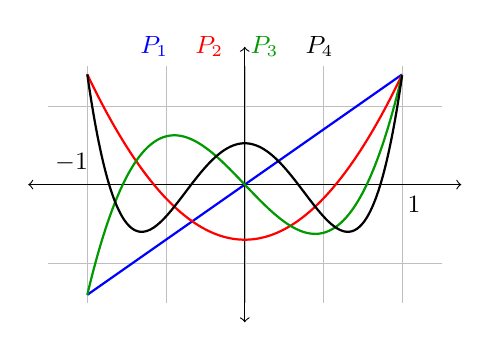
\begin{tikzpicture}
    \draw[ultra thin,color=lightgray] (-2.5,-1.5) grid (2.5,1.5);
    \draw[<->] (-2.75,0) -- (2.75,0);
    \draw[<->] (0,-1.75) -- (0,1.75);
    % x scaled by 2, y scaled by 1.4
    \draw [thick, samples=100,smooth, color=blue] plot[variable=\t, domain=-1:1] ({2*\t},{1.4*\t});
    \draw [thick, samples=100,smooth, color=red] plot[variable=\t, domain=-1:1] ({2*\t},{1.4*0.5*(3*\t*\t - 1)});
    \draw [thick, samples=100,smooth, color=green!60!black] plot[variable=\t, domain=-1:1] ({2*\t},{1.4*0.5*(5*\t*\t*\t - 3*\t)});
    \draw [thick, samples=120,smooth, color=black] plot[variable=\t, domain=-1:1] ({2*\t},{1.4*0.125*(35*\t*\t*\t*\t - 30*\t*\t + 3)});
    \node[color=blue] at (-1.15, 1.75) {\small $P_1$};
    \node[color=red] at (-0.45, 1.75) {\small $P_2$};
    \node[color=green!60!black] at (0.25, 1.75) {\small $P_3$};
    \node[color=black] at (0.95, 1.75) {\small $P_4$};
    \node at (2.15, -0.25) {\small $1$};
    \node at (-2.2, 0.28) {\small $-1$};
\end{tikzpicture}
\end{center}

Because they are eigenfunctions of a self-adjoint problem with distinct eigenvalues, the Legendre polynomials are automatically orthogonal:
$$
\int_{-1}^1 P_n(x) P_m(x) \dd x = 0 \quad \text{for } n \neq m,
$$
and one can compute the normalisation
$$
\int_{-1}^1 P_n(x)^2 \dd x = \frac{2}{2n + 1}.
$$

There are a number of useful ways to generate the $P_\ell$ without solving the recursion each time. There is \vocab{Rodrigues' formula}
$$
P_\ell(x) = \frac{1}{2^\ell \ell!} \frac{\dd^\ell}{\dd x^\ell} (x^2 - 1)^\ell,
$$
and the \vocab{generating function}
$$
\frac{1}{\sqrt{1 - 2xt + t^2}} = \sum_{\ell = 0}^{\infty} P_\ell(x) t^\ell,
$$
which we shall derive when we study Laplace's equation (it is secretly the potential of a point charge). There are also recursion relations such as
\begin{align*}
(\ell + 1) P_{\ell + 1}(x) &= (2\ell + 1) x P_\ell(x) - \ell P_{\ell - 1}(x), \\
\text{and} \quad (2 \ell + 1) P_\ell(x) &= \frac{\dd}{\dd x}\left[P_{\ell + 1}(x) - P_{\ell - 1}(x)\right].
\end{align*}

Since the Legendre polynomials form a complete orthogonal set on $[-1, 1]$, any well-behaved $f$ on $[-1, 1]$ has a \vocab{Fourier--Legendre series}
$$
f(x) = \sum_{\ell = 0}^{\infty} a_\ell P_\ell(x), \quad a_\ell = \frac{2 \ell + 1}{2} \int_{-1}^1 f(x) P_\ell(x) \dd x.
$$
Note that unlike Fourier series, no periodicity of $f$ is required -- the boundary conditions here were just finiteness.

\subsection{Solving Inhomogeneous ODEs by Eigenfunction Expansion}

We now have everything needed to run the `self-adjoint matrix' strategy in general. Suppose we want to solve
$$
\mathcal{L} y = f(x) = w(x) F(x)
$$
on $[a, b]$ with homogeneous boundary conditions, where $\mathcal{L}$ is in Sturm--Liouville form with eigenfunctions $\mathcal{L} y_n = \lambda_n w y_n$. Expand both the solution and the source:
$$
y(x) = \sum_n c_n y_n(x), \quad F(x) = \sum_n a_n y_n(x),
$$
where the $a_n$ are known:
$$
a_n = \frac{\int_a^b w F y_n \dd x}{\int_a^b w y_n^2 \dd x}.
$$
Substituting,
$$
\mathcal{L} y = \sum_n c_n \mathcal{L} y_n = w \sum_n c_n \lambda_n y_n = w \sum_n a_n y_n,
$$
and by orthogonality we can equate coefficients, giving $c_n = a_n / \lambda_n$. So
$$
y(x) = \sum_{n = 1}^{\infty} \frac{a_n}{\lambda_n} y_n(x),
$$
provided no $\lambda_n = 0$.

A common variant includes a driving term at fixed `frequency': for the equation
$$
\mathcal{L}y - \tilde{\lambda} w y = f(x),
$$
with $\tilde{\lambda}$ a fixed constant, exactly the same computation gives
$$
y(x) = \sum_{n = 1}^{\infty} \frac{a_n}{\lambda_n - \tilde{\lambda}} y_n(x).
$$
Notice what happens as $\tilde{\lambda}$ approaches an eigenvalue $\lambda_n$ with $a_n \neq 0$: the response blows up. This is \emph{resonance}, seen here in complete generality.

\subsubsection*{Towards Green's Functions}

Let's rewrite our solution in a rather suggestive way. Substituting the integral formula for $a_n$ into the solution, and writing $N_n = \int_a^b w y_n^2 \dd x$,
$$
y(x) = \sum_{n = 1}^{\infty} \frac{y_n(x)}{\lambda_n N_n} \int_a^b w(\xi) F(\xi) y_n(\xi) \dd \xi
= \int_a^b \underbrace{\left(\sum_{n = 1}^{\infty} \frac{y_n(x) y_n(\xi)}{\lambda_n N_n}\right)}_{G(x, \xi)} \underbrace{w(\xi) F(\xi)}_{f(\xi)} \dd \xi.
$$
That is,
$$
y(x) = \int_a^b G(x, \xi) f(\xi) \dd \xi, \quad \text{where} \quad G(x, \xi) = \sum_{n = 1}^{\infty} \frac{y_n(x) y_n(\xi)}{\lambda_n N_n}.
$$
The function $G$, called the \vocab{Green's function}, depends only on $\mathcal{L}$ and the boundary conditions -- \emph{not} on the source $f$. It acts as a kind of inverse operator
$$
\mathcal{L}^{-1} = \int_a^b \dd \xi \, G(x, \xi),
$$
in perfect analogy with $\vv x = A^{-1} \vv b$ for matrices. We will return to Green's functions in earnest later in the course, where we will construct them directly (without infinite sums) and interpret them as responses to point sources.

\section{The Wave Equation}

It's time to put our machinery to work on an actual partial differential equation. The star of this section is the \vocab{wave equation}
$$
\frac{1}{c^2} \frac{\partial^2 y}{\partial t^2} = \frac{\partial^2 y}{\partial x^2},
$$
which governs (among many other things) the small vibrations of a stretched string.

\subsection{Waves on an Elastic String}

Let's first see where the equation comes from. Consider a stretched elastic string with tension $T$ and linear mass density $\mu$, with ends fixed at $x = 0$ and $x = L$, and let $y(x, t)$ be the (small) transverse displacement. We make the key assumption that displacements are small, in the sense that $\abs{\partial y / \partial x} \ll 1$.

Consider the segment of string between $x$ and $x + \delta x$. Tension pulls the segment along the string at each end: at the right end at a small angle $\theta_2$ to the horizontal, and at the left end at angle $\theta_1$.
Resolving horizontally, since the string doesn't move sideways,
$$
T_1 \cos \theta_1 = T_2 \cos \theta_2,
$$
and as $\cos \theta = 1 + O(\theta^2)$, the tension is uniform along the string to leading order: $T_1 \approx T_2 = T$.
Resolving vertically, using $\sin \theta \approx \tan \theta = \partial y/\partial x$ for small angles, the net transverse force is
$$
T \left(\left.\frac{\partial y}{\partial x}\right|_{x + \delta x} - \left.\frac{\partial y}{\partial x}\right|_x \right) \approx T \frac{\partial^2 y}{\partial x^2} \delta x.
$$
The mass of the segment is $\mu \, \delta x$, so Newton's second law (including gravity, with $g$ downwards) gives
$$
\mu \, \delta x \frac{\partial^2 y}{\partial t^2} = T \frac{\partial^2 y}{\partial x^2}\delta x - g \mu\, \delta x.
$$
For a taut string the tension term utterly dominates gravity, so we neglect $g$, and dividing through by $\mu \, \delta x$ we obtain the wave equation
$$
\frac{\partial^2 y}{\partial t^2} = c^2 \frac{\partial^2 y}{\partial x^2}, \quad \text{where } c = \sqrt{\frac{T}{\mu}}
$$
is the \vocab{wave speed}. Alongside the boundary conditions $y(0, t) = y(L, t) = 0$, a full problem also specifies initial conditions
$$
y(x, 0) = p(x), \quad \frac{\partial y}{\partial t}(x, 0) = q(x).
$$
Note that we need \emph{two} initial conditions, since the equation is second order in time.

\subsection{Separation of Variables}

Our main technique for solving the wave equation (and later the diffusion and Laplace equations) is \vocab{separation of variables}: we look for solutions in the special product form
$$
y(x, t) = X(x) T(t).
$$
Substituting into the wave equation gives $\frac{1}{c^2} X \ddot{T} = X'' T$, and dividing by $XT$,
$$
\frac{1}{c^2} \frac{\ddot{T}}{T} = \frac{X''}{X}.
$$
Now here's the trick: the left-hand side depends only on $t$, and the right-hand side only on $x$. The only way a function of $t$ can equal a function of $x$ for all $x$ and $t$ is if both are constant. Calling this \vocab{separation constant} $-\lambda$, we get two ODEs
$$
X'' + \lambda X = 0, \quad \ddot{T} + \lambda c^2 T = 0.
$$

We solve the spatial problem first, since it carries the boundary conditions $X(0) = X(L) = 0$. This is exactly a Sturm--Liouville eigenvalue problem! Let's check the possible signs of $\lambda$.
\begin{enumerate}[label=(\roman*)]
    \item If $\lambda < 0$, write $\chi^2 = -\lambda$; then $X = C \cosh \chi x + D \sinh \chi x$, and the boundary conditions force $C = D = 0$.
    \item If $\lambda = 0$, then $X = Ax + B$, and again only the trivial solution survives.
    \item If $\lambda > 0$, then $X = A \cos(\sqrt{\lambda} x) + B \sin(\sqrt{\lambda}x)$. Now $X(0) = 0$ gives $A = 0$, and $X(L) = 0$ requires $\sin (\sqrt{\lambda} L) = 0$, i.e.\ $\sqrt{\lambda} L = n \pi$.
\end{enumerate}
So we find the eigenfunctions and eigenvalues
$$
X_n(x) = \sin \frac{n \pi x}{L}, \quad \lambda_n = \left(\frac{n \pi}{L}\right)^2, \quad n = 1, 2, \dots.
$$

These spatial profiles are called the \vocab{normal modes} of the string: the shape in $x$ is frozen, and only the amplitude oscillates in time. The $n = 1$ mode is the \vocab{fundamental}, and higher modes are \emph{overtones}, with $n - 1$ stationary points (`nodes') in the interior.

\begin{center}
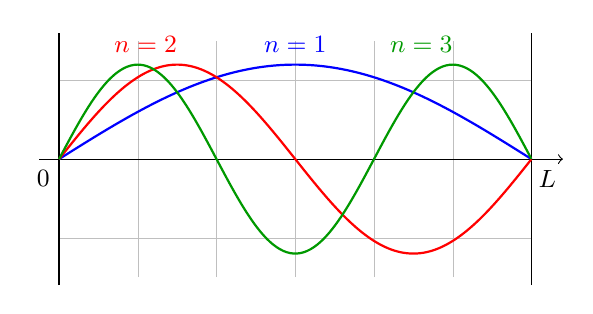
\begin{tikzpicture}
    \draw[ultra thin,color=lightgray] (0,-1.5) grid (6,1.5);
    \draw[->] (-0.25,0) -- (6.4,0);
    \draw (0,-1.6) -- (0,1.6);
    \draw (6,-1.6) -- (6,1.6);
    \draw [thick, samples=100,smooth, color=blue] plot[variable=\t, domain=0:6] ({\t},{1.2*sin(30*\t)});
    \draw [thick, samples=100,smooth, color=red] plot[variable=\t, domain=0:6] ({\t},{1.2*sin(60*\t)});
    \draw [thick, samples=140,smooth, color=green!60!black] plot[variable=\t, domain=0:6] ({\t},{1.2*sin(90*\t)});
    \node[color=blue] at (3, 1.45) {\small $n = 1$};
    \node[color=red] at (1.1, 1.45) {\small $n = 2$};
    \node[color=green!60!black] at (4.6, 1.45) {\small $n = 3$};
    \node at (-0.2, -0.25) {\small $0$};
    \node at (6.2, -0.25) {\small $L$};
\end{tikzpicture}
\end{center}

With $\lambda_n$ fixed, the temporal equation $\ddot{T} + (n \pi c/L)^2 T = 0$ has solutions
$$
T_n(t) = C_n \cos \frac{n \pi c t}{L} + D_n \sin \frac{n \pi c t}{L},
$$
so each normal mode oscillates at angular frequency $\omega_n = n \pi c /L$. Superposing everything (the equation is linear!), the general solution satisfying the boundary conditions is
$$
y(x, t) = \sum_{n = 1}^{\infty} \left(C_n \cos \frac{n \pi c t}{L} + D_n \sin \frac{n \pi c t}{L}\right) \sin \frac{n \pi x }{L}.
$$

It remains to impose the initial conditions. Setting $t = 0$,
$$
y(x, 0) = p(x) = \sum_{n = 1}^{\infty} C_n \sin \frac{n \pi x}{L},
$$
which is precisely a half-range Fourier sine series, and differentiating in time first,
$$
\frac{\partial y}{\partial t}(x, 0) = q(x) = \sum_{n = 1}^{\infty} \frac{n \pi c}{L} D_n \sin \frac{n \pi x}{L}.
$$
So by our Fourier coefficient formulas,
$$
C_n = \frac{2}{L} \int_0^L p(x) \sin \frac{n \pi x}{L} \dd x, \quad D_n = \frac{2}{n \pi c} \int_0^L q(x) \sin \frac{n \pi x}{L} \dd x.
$$

\begin{example}[The Plucked String]
    Take $L = 1$ and pluck the string at the point $x = \xi$: the initial condition is the `see-saw' shape
    $$
    y(x, 0) = p(x) = \begin{cases}
        x (1 - \xi) &\mbox{if } 0 \leq x < \xi, \\
        \xi (1 - x) &\mbox{if } \xi \leq x < 1,
    \end{cases}
    $$
    released from rest, $q(x) = 0$. We computed the Fourier series of this function before:
    $$
    C_n = \frac{2 \sin n \pi \xi}{(n \pi)^2}, \quad D_n = 0,
    $$
    so the subsequent motion is
    $$
    y(x, t) = \sum_{n = 1}^{\infty} \frac{2 \sin n \pi \xi}{(n \pi)^2} \sin (n \pi x) \cos( n \pi c t).
    $$
    Notice that if you pluck at the midpoint $\xi = 1/2$, all the even harmonics vanish -- plucking position controls the timbre.
\end{example}

Summarising, the general strategy of separation of variables is:
\begin{enumerate}
    \item write down the linear PDE with its boundary and initial conditions;
    \item separate variables to get decoupled ODEs;
    \item impose the homogeneous boundary conditions to find the eigenvalues and eigenfunctions;
    \item use the separation constants to solve for the remaining variables;
    \item superpose the separable solutions into a general series solution;
    \item fix the coefficients using the initial (or remaining boundary) conditions.
\end{enumerate}
This exact recipe will reappear for the diffusion equation and Laplace's equation.

\subsection{d'Alembert's Solution and Characteristics}

There's a completely different way of looking at the wave equation, which doesn't involve series at all. Using the sum formulas $\sin A \cos B = \frac{1}{2}(\sin(A - B) + \sin(A + B))$ and so on, each standing wave term in our series solution splits as
\begin{align*}
    y(x, t) &= \frac{1}{2}\sum_{n = 1}^{\infty} \left[C_n \sin \frac{n \pi}{L}(x - ct) + D_n \cos \frac{n \pi}{L}(x - ct)\right] \\
    &\quad + \frac{1}{2}\sum_{n = 1}^{\infty} \left[C_n \sin \frac{n \pi}{L}(x + ct) - D_n \cos \frac{n \pi}{L}(x + ct)\right],
\end{align*}
that is, everything is a function of $x - ct$ plus a function of $x + ct$. This is no accident. Changing variables to $u = x - ct$, $v = x + ct$ transforms the wave equation into
$$
\frac{\partial^2 y}{\partial u \, \partial v} = 0,
$$
(we will verify this carefully when we study characteristics in general), which integrates immediately to give
$$
y(x, t) = f(x - ct) + g(x + ct)
$$
for arbitrary functions $f$ and $g$: a right-moving wave and a left-moving wave, each travelling at speed $c$ with unchanging shape.

Let's fit $f$ and $g$ to initial data on the whole line, $y(x, 0) = p(x)$ and $y_t(x, 0) = q(x)$. At $t = 0$,
$$
f(x) + g(x) = p(x), \quad -c f'(x) + c g'(x) = q(x).
$$
Differentiating the first equation and combining with the second,
$$
g'(x) = \frac{1}{2}\left(p'(x) + \frac{q(x)}{c}\right), \quad f'(x) = \frac{1}{2}\left(p'(x) - \frac{q(x)}{c}\right),
$$
and integrating (the constants of integration cancel in $f + g$) we arrive at \vocab{d'Alembert's solution}
$$
y(x, t) = \frac{1}{2}\left[p(x - ct) + p(x + ct)\right] + \frac{1}{2c} \int_{x - ct}^{x + ct} q(s) \dd s.
$$
In particular, a string released from rest ($q = 0$) evolves as $y = \frac{1}{2}[p(x - ct) + p(x + ct)]$ -- the initial shape splits into two half-size copies moving apart.

d'Alembert's formula makes a physically important point manifest: the solution at position $x$ and time $t$ depends only on the initial data in the interval $[x - ct, x + ct]$. Information propagates no faster than speed $c$.

\begin{center}
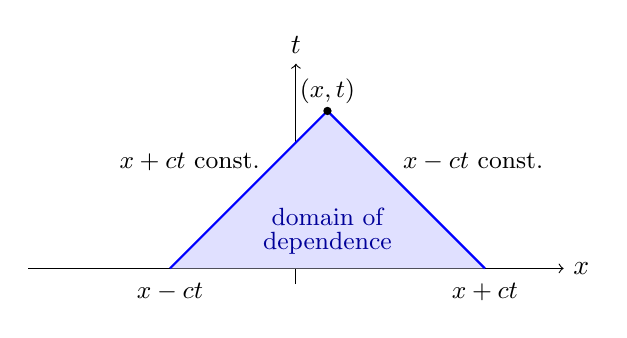
\begin{tikzpicture}
    % x-t plane, domain of dependence
    \draw[->] (-3.4,0) -- (3.4,0) node[right] {$x$};
    \draw[->] (0,-0.2) -- (0,2.6) node[above] {$t$};
    \fill[blue!12] (0.4,2) -- (-1.6,0) -- (2.4,0) -- cycle;
    \draw[thick, color=blue] (0.4,2) -- (-1.6,0);
    \draw[thick, color=blue] (0.4,2) -- (2.4,0);
    \fill (0.4,2) circle (1.5pt);
    \node at (0.4, 2.25) {\small $(x, t)$};
    \node at (-1.6, -0.3) {\small $x - ct$};
    \node at (2.4, -0.3) {\small $x + ct$};
    \node at (0.4, 0.65) {\small \color{blue!60!black} domain of};
    \node at (0.4, 0.32) {\small \color{blue!60!black} dependence};
    \node at (-1.35, 1.35) {\small $x + ct$ const.};
    \node at (2.25, 1.35) {\small $x - ct$ const.};
\end{tikzpicture}
\end{center}

The lines $x \pm ct = \text{const}$ are called the \vocab{characteristics} of the wave equation. The shaded triangle is the \vocab{domain of dependence} of the point $(x, t)$; dually, initial data at a point $(x_0, 0)$ can only ever influence the forward wedge $\{(x,t) : \abs{x - x_0} \leq ct\}$, its \vocab{range of influence}.

\subsection{Energy of Oscillations}

A vibrating string carries energy, and tracking it is both physically illuminating and a nice application of Parseval. The kinetic energy is
$$
\text{KE} = \frac{1}{2}\mu \int_0^L \left(\frac{\partial y}{\partial t}\right)^2 \dd x,
$$
and the potential energy is the work done stretching the string against tension. The stretched length element is $\sqrt{1 + (\partial y/\partial x)^2}\dd x$, so
$$
\text{PE} = T \int_0^L \left(\sqrt{1 + \left(\frac{\partial y}{\partial x}\right)^2} - 1\right) \dd x \approx \frac{T}{2} \int_0^L \left(\frac{\partial y}{\partial x}\right)^2 \dd x,
$$
using the small-slope assumption. Hence, using $c^2 = T/\mu$, the total energy is
$$
E = \frac{1}{2} \mu \int_0^L \left[\left(\frac{\partial y}{\partial t}\right)^2 + c^2 \left(\frac{\partial y}{\partial x}\right)^2\right] \dd x.
$$
Substituting our normal mode expansion and integrating using orthogonality (all the cross terms die, and $\int_0^L \sin^2 = \int_0^L \cos^2 = L/2$),
$$
E = \frac{1}{4} \mu \sum_{n = 1}^{\infty} \frac{n^2 \pi^2 c^2}{L}\left(C_n^2 + D_n^2\right),
$$
where the time dependence has cancelled via $\cos^2 + \sin^2 = 1$. So the energy is \emph{constant in time}, as it should be, and moreover it decomposes as a sum over normal modes -- each mode holds its own energy and never trades it with the others. This is really Parseval's theorem wearing a physics costume.

\subsection{Wave Reflection and Transmission}

Let's briefly consider what happens when a travelling wave meets a change in the medium. A \vocab{simple harmonic travelling wave} has the form
$$
y = \re\left[A e^{i \omega (t - x/c)}\right] = \abs{A} \cos\left(\omega(t - x/c) + \phi\right),
$$
where the phase $\phi = \arg A$ and the wavelength is $2 \pi c / \omega$.

Suppose the density of the string jumps at $x = 0$:
$$
\mu = \begin{cases}
    \mu_- &\mbox{if } x < 0, \\
    \mu_+ &\mbox{if } x > 0,
\end{cases}
\quad \text{so} \quad
c_\pm = \sqrt{T / \mu_\pm},
$$
with the tension $T$ constant throughout. Send in a wave $A e^{i \omega (t - x/c_-)}$ from the left. At the join, some of the wave is reflected, $B e^{i \omega (t + x /c_-)}$, and some is transmitted, $D e^{i \omega (t - x/c_+)}$. Note all three waves must share the frequency $\omega$ to have any hope of matching at $x = 0$ for all time.

The physical matching conditions at $x = 0$ are:
\begin{enumerate}[label=(\roman*)]
    \item $y$ is continuous (the string doesn't break), giving $A + B = D$;
    \item the transverse force $T \partial y/\partial x$ is continuous (else a massless point would suffer infinite acceleration), giving
    $$
    \frac{-i \omega A}{c_-} + \frac{i \omega B}{c_-} = \frac{-i \omega D}{c_+}.
    $$
\end{enumerate}
Solving these two equations,
$$
D = \frac{2 c_+}{c_+ + c_-} A, \quad B = \frac{c_+ - c_-}{c_+ + c_-} A.
$$

Various limits of this formula are illuminating:
\begin{enumerate}[label=(\roman*)]
    \item If $c_- = c_+$ (no jump at all), then $D = A$ and $B = 0$: full transmission.
    \item If $\mu_+/\mu_- \rightarrow \infty$, the right half becomes infinitely heavy -- effectively a fixed end (a \emph{Dirichlet} boundary condition at $x = 0$). Then $c_+/c_- \rightarrow 0$, so $D = 0$ and $B = -A$: total reflection with phase flipped by $\pi$.
    \item If $\mu_+ / \mu_- \rightarrow 0$, the right half is massless -- a free end (a \emph{Neumann} condition). Then $c_+ / c_- \rightarrow \infty$, giving $B = A$: total reflection in phase (and the formula gives $D = 2A$, but this carries no energy as $\mu_+ \to 0$).
\end{enumerate}

\subsection{The Wave Equation in Plane Polar Coordinates}

So far our string has been one-dimensional. Let's now solve the two-dimensional wave equation on the unit disc -- physically, a circular drum. We want $u(r, \theta, t)$ satisfying
$$
\frac{1}{c^2} \frac{\partial^2 u}{\partial t^2} = \nabla^2 u,
$$
with boundary condition $u(1, \theta, t) = 0$ (the drum skin is clamped at the rim) and initial conditions
$$
u(r, \theta, 0) = \phi(r, \theta), \quad \frac{\partial u}{\partial t}(r, \theta, 0) = \psi(r, \theta).
$$

We separate off time first: substituting $u = T(t) V(r, \theta)$ gives
$$
\ddot{T} + \lambda c^2 T = 0, \quad \nabla^2 V + \lambda V = 0.
$$
In plane polars the spatial equation reads
$$
\frac{\partial^2 V}{\partial r^2} + \frac{1}{r}\frac{\partial V}{\partial r} + \frac{1}{r^2} \frac{\partial^2 V}{\partial \theta^2} + \lambda V = 0,
$$
and separating again with $V = R(r) \Theta(\theta)$,
$$
\Theta'' + \mu \Theta = 0, \quad r^2 R'' + r R' + (\lambda r^2 - \mu) R = 0.
$$
On the disc, $\Theta$ must be $2\pi$-periodic, which forces $\mu = m^2$ with $m \in \N$, and
$$
\Theta_m(\theta) = A_m \cos m \theta + B_m \sin m \theta.
$$

\subsection{Bessel's Equation}

Now for the radial equation. Dividing by $r$ puts it in Sturm--Liouville form,
$$
-\left(r R'\right)' + \frac{m^2}{r} R = \lambda r R,
$$
with $p(r) = r$, $q(r) = m^2/r$ and weight $w(r) = r$. Note $p(0) = 0$, so $r = 0$ is a singular point, and the correct `boundary condition' there is just that $R$ stays bounded; at the rim we have $R(1) = 0$. Substituting $z = \sqrt{\lambda} r$ tidies away $\lambda$ and yields \vocab{Bessel's equation}
$$
z^2 \frac{\dd^2 R}{\dd z^2} + z \frac{\dd R}{\dd z} + (z^2 - m^2) R = 0.
$$

Since $z = 0$ is a regular singular point, we solve by Frobenius' method, trying $R = z^p \sum_{n \geq 0} a_n z^n$. The lowest power of $z$ gives the indicial equation
$$
p^2 - m^2 = 0 \implies p = \pm m.
$$
Taking the regular root $p = m$, comparing coefficients of $z^{n + m}$ gives the recursion
$$
\left((n + m)^2 - m^2\right) a_n + a_{n - 2} = 0 \implies a_n = \frac{-a_{n - 2}}{n (n + 2m)},
$$
so only even $n$ appear, and iterating,
$$
a_{2k} = \frac{(-1)^k a_0}{2^{2k} k! (m + 1)(m+2)\cdots(m + k)}.
$$
With the conventional normalisation $a_0 = 1/(2^m m!)$ we obtain the \vocab{Bessel function of the first kind}
$$
J_m(z) = \left(\frac{z}{2}\right)^m \sum_{k = 0}^{\infty} \frac{(-1)^k}{k! \, (k + m)!} \left(\frac{z}{2}\right)^{2k}.
$$
The second solution (from $p = -m$, suitably interpreted) is the Bessel function of the second kind $Y_m(z)$, which diverges as $z \rightarrow 0$; boundedness at the origin will always eliminate it for us.

\begin{center}
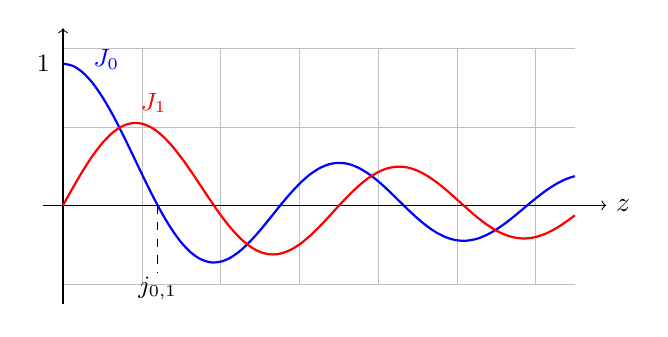
\begin{tikzpicture}
    \draw[ultra thin,color=lightgray] (0,-1) grid (6.5,2);
    \draw[->] (-0.25,0) -- (6.9,0) node[right] {$z$};
    \draw[->] (0,-1.25) -- (0,2.25);
    % x = z/2, y = 1.8 J(z)
    \draw [thick, smooth, color=blue] plot coordinates {(0.000,1.800) (0.125,1.772) (0.250,1.689) (0.375,1.556) (0.500,1.377) (0.625,1.163) (0.750,0.921) (0.875,0.664) (1.000,0.403) (1.125,0.149) (1.250,-0.087) (1.375,-0.295) (1.500,-0.468) (1.625,-0.599) (1.750,-0.684) (1.875,-0.723) (2.000,-0.715) (2.125,-0.665) (2.250,-0.577) (2.375,-0.459) (2.500,-0.320) (2.625,-0.168) (2.750,-0.012) (2.875,0.137) (3.000,0.271) (3.125,0.384) (3.250,0.468) (3.375,0.521) (3.500,0.540) (3.625,0.526) (3.750,0.479) (3.875,0.405) (4.000,0.309) (4.125,0.197) (4.250,0.075) (4.375,-0.047) (4.500,-0.163) (4.625,-0.265) (4.750,-0.349) (4.875,-0.409) (5.000,-0.443) (5.125,-0.448) (5.250,-0.426) (5.375,-0.378) (5.500,-0.308) (5.625,-0.221) (5.750,-0.122) (5.875,-0.017) (6.000,0.086) (6.125,0.182) (6.250,0.264) (6.375,0.329) (6.500,0.372)};
    \draw [thick, smooth, color=red] plot coordinates {(0.000,0.000) (0.125,0.223) (0.250,0.436) (0.375,0.629) (0.500,0.792) (0.625,0.919) (0.750,1.004) (0.875,1.044) (1.000,1.038) (1.125,0.987) (1.250,0.895) (1.375,0.767) (1.500,0.610) (1.625,0.434) (1.750,0.247) (1.875,0.060) (2.000,-0.119) (2.125,-0.280) (2.250,-0.416) (2.375,-0.521) (2.500,-0.590) (2.625,-0.621) (2.750,-0.615) (2.875,-0.572) (3.000,-0.498) (3.125,-0.397) (3.250,-0.277) (3.375,-0.145) (3.500,-0.008) (3.625,0.123) (3.750,0.243) (3.875,0.345) (4.000,0.422) (4.125,0.472) (4.250,0.492) (4.375,0.481) (4.500,0.442) (4.625,0.376) (4.750,0.290) (4.875,0.189) (5.000,0.078) (5.125,-0.034) (5.250,-0.142) (5.375,-0.238) (5.500,-0.318) (5.625,-0.377) (5.750,-0.411) (5.875,-0.420) (6.000,-0.402) (6.125,-0.361) (6.250,-0.298) (6.375,-0.218) (6.500,-0.127)};
    \node[color=blue] at (0.55, 1.85) {\small $J_0$};
    \node[color=red] at (1.15, 1.3) {\small $J_1$};
    \draw[dashed] (1.203,0) -- (1.203,-0.85);
    \node at (1.203, -1.05) {\small $j_{0,1}$};
    \node at (-0.25, 1.8) {\small $1$};
\end{tikzpicture}
\end{center}

For small $z$, the leading behaviour is $J_0(z) \approx 1$ and $J_m(z) \approx \frac{1}{m!}(z/2)^m$. For large $z$, the Bessel functions become decaying oscillations:
$$
J_m(z) \approx \sqrt{\frac{2}{\pi z}} \cos \left(z - \frac{m \pi}{2} - \frac{\pi}{4}\right).
$$
In particular each $J_m$ has infinitely many positive zeros. We write $j_{mn}$ for the $n$th positive zero of $J_m$; from the asymptotic form,
$$
j_{mn} \approx n \pi + \frac{m \pi}{2} - \frac{\pi}{4} \quad \text{for large } n.
$$
The zeros play exactly the role that $n \pi$ played for $\sin$: they are what the boundary condition will latch onto. (For reference, $j_{01} \approx 2.405$.)

\subsection{The Vibrating Drum}

Let's assemble the solution of the drum problem. The radial solutions are $R(r) = A J_m(\sqrt{\lambda} r) + B Y_m(\sqrt{\lambda}r)$; boundedness at the centre gives $B = 0$, and the clamped rim $R(1) = 0$ requires
$$
J_m(\sqrt{\lambda}) = 0 \implies \sqrt{\lambda} = j_{mn}, \quad \text{i.e. } \lambda_{mn} = j_{mn}^2.
$$
So the spatial normal modes of the drum are
$$
V_{mn}(r, \theta) = \left(A_{mn} \cos m \theta + B_{mn} \sin m \theta\right) J_m (j_{mn} r),
$$
with frequencies $\omega_{mn} = j_{mn} c$. The mode $(m, n)$ has $m$ nodal diameters and $n - 1$ interior nodal circles.

\begin{center}
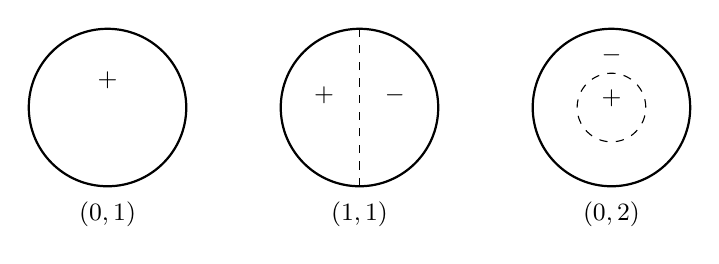
\begin{tikzpicture}
    % mode (0,1)
    \draw[thick] (0,0) circle (1);
    \node at (0, 0.35) {\small $+$};
    \node at (0,-1.35) {\small $(0,1)$};
    % mode (1,1)
    \begin{scope}[shift={(3.2,0)}]
        \draw[thick] (0,0) circle (1);
        \draw[dashed] (0,-1) -- (0,1);
        \node at (-0.45, 0.15) {\small $+$};
        \node at (0.45, 0.15) {\small $-$};
        \node at (0,-1.35) {\small $(1,1)$};
    \end{scope}
    % mode (0,2)
    \begin{scope}[shift={(6.4,0)}]
        \draw[thick] (0,0) circle (1);
        \draw[dashed] (0,0) circle (0.4359);
        \node at (0, 0.12) {\small $+$};
        \node at (0, 0.66) {\small $-$};
        \node at (0,-1.35) {\small $(0,2)$};
    \end{scope}
\end{tikzpicture}
\end{center}

The full solution is a superposition over all modes,
\begin{align*}
u(r, \theta, t) = \sum_{m = 0}^{\infty} \sum_{n = 1}^{\infty} J_m(j_{mn} r) \Big[&\left(A_{mn} \cos m\theta + B_{mn} \sin m \theta\right) \cos (j_{mn} c t) \\
&+ \left(C_{mn} \cos m \theta + D_{mn} \sin m \theta\right) \sin (j_{mn} c t)\Big],
\end{align*}
and the coefficients are fixed by the initial conditions using the orthogonality of $\cos m\theta$, $\sin m \theta$ \emph{and} of the Bessel functions themselves. Indeed, since the $J_m(j_{mn} r)$ for fixed $m$ are eigenfunctions of a Sturm--Liouville problem with weight $r$, we have
$$
\int_0^1 J_m(j_{mn} r) J_m (j_{mk}r)\, r \dd r = \frac{1}{2}\left[J_{m + 1}(j_{mn})\right]^2 \delta_{nk}.
$$

\begin{example}[A Radially Symmetric Drum Strike]
    Suppose the drum starts at rest from the radially symmetric profile $u(r, \theta, 0) = \phi(r) = 1 - r^2$.
    By symmetry only the $m = 0$ modes are excited, and starting from rest kills the $\sin(j_{0n}ct)$ terms, so
    $$
    u(r, \theta, t) = \sum_{n = 1}^{\infty} A_{0n} J_0 (j_{0n} r) \cos (j_{0n} c t),
    $$
    where
    $$
    A_{0n} = \frac{\int_0^1 (1 - r^2) J_0(j_{0n} r)\, r \dd r}{\frac{1}{2}J_1(j_{0n})^2}.
    $$
    Working out the integral using Bessel recursion relations, one finds
    $$
    A_{0n} = \frac{8 J_2(j_{0n})}{j_{0n}^2 J_1(j_{0n})^2}.
    $$
    The fundamental frequency of a drum of diameter $d$ is $\omega = j_{01}c \cdot 2/d \approx 4.8\, c/d$, compared with $\pi c/d \approx 3.1\, c/d$ for a string of length $d$. Moreover the overtone frequencies $j_{0n}$ are \emph{not} integer multiples of $j_{01}$ -- which is why a drum sounds like a thud rather than a note.
\end{example}

\section{The Diffusion Equation}

The next equation in our collection is the \vocab{diffusion equation} (or \emph{heat equation})
$$
\frac{\partial \theta}{\partial t} = D \nabla^2 \theta,
$$
which describes how heat, or the concentration of diffusing particles, spreads out over time. It is first order in time -- a fact with real consequences, as we'll see: unlike the wave equation, diffusion has an arrow of time.

\subsection{Deriving the Diffusion Equation}

\subsubsection*{Via Fourier's Law}

Consider the temperature $\theta(\vv x, t)$ in a conducting body. The heat energy in a fixed volume $V$ is
$$
Q = \int_V c_V \rho \, \theta \dd V,
$$
where $c_V$ is the specific heat and $\rho$ the density, so
$$
\frac{\dd Q}{\dd t} = \int_V c_V \rho \frac{\partial \theta}{\partial t} \dd V.
$$
Empirically, heat flows from hot to cold at a rate proportional to the temperature gradient. This is \vocab{Fourier's law}:
$$
\vv q = -k \nabla \theta,
$$
where $\vv q$ is the heat flux and $k$ the conductivity. The heat leaving $V$ through its boundary is then
$$
-\frac{\dd Q}{\dd t} = \int_{\partial V} \vv q \cdot \hat{\vv n} \dd S = \int_{\partial V} (-k \nabla \theta) \cdot \hat{\vv n} \dd S = -\int_V k \nabla^2 \theta \dd V,
$$
using the divergence theorem. Equating the two expressions,
$$
\int_V \left(c_V \rho \frac{\partial \theta}{\partial t} - k \nabla^2 \theta \right) \dd V = 0,
$$
and since $V$ was arbitrary, the integrand must vanish identically. Writing $D = k /(c_V \rho)$, the \vocab{diffusion constant} (or diffusivity), we get the diffusion equation
$$
\frac{\partial \theta}{\partial t} = D \nabla^2 \theta.
$$

\subsubsection*{Via Random Walks}

There is a rather different derivation which explains why the same equation governs diffusing gas particles. Suppose a particle takes a random step of displacement $\xi$ every time interval $\Delta t$, where $\xi$ is drawn from a probability density $p(\xi)$ with no directional bias, $\langle \xi \rangle = \int \xi p(\xi) \dd \xi = 0$.
If $P(x, N \Delta t)$ is the probability density for the particle's position after $N$ steps, then conditioning on the last step,
$$
P(x, (N + 1)\Delta t) = \int_{-\infty}^{\infty} p(\xi) P(x - \xi, N \Delta t) \dd \xi.
$$
Taylor expanding $P$ in its first argument about $x$,
$$
P(x, (N+1)\Delta t) \approx P(x, N \Delta t) - \langle \xi \rangle \frac{\partial P}{\partial x} + \frac{\langle \xi^2 \rangle}{2} \frac{\partial^2 P}{\partial x^2} = P(x, N \Delta t) + \frac{\langle \xi^2 \rangle}{2} \frac{\partial^2 P}{\partial x^2},
$$
using $\int p = 1$ and $\langle \xi \rangle = 0$. So provided the variance scales with the time step as $\langle \xi^2 \rangle = 2 D \Delta t$, taking $\Delta t$ small gives
$$
\frac{\partial P}{\partial t} = D \frac{\partial^2 P}{\partial x^2},
$$
the diffusion equation again. The scaling $\langle \xi^2 \rangle \propto \Delta t$ is the fingerprint of diffusion: distance travelled grows like $\sqrt{t}$, not $t$.

\subsection{Similarity Solutions}

That $\sqrt{t}$ scaling suggests that the combination $x/\sqrt{t}$ might be a natural variable, and indeed the diffusion equation admits \vocab{similarity solutions} depending only on the dimensionless variable
$$
\eta = \frac{x}{2 \sqrt{D t}}.
$$
Let's look for a solution $\theta(x, t) = \theta(\eta)$. Using the chain rule,
$$
\frac{\partial \theta}{\partial t} = -\frac{1}{2}\frac{\eta}{t} \theta'(\eta), \quad
D \frac{\partial^2 \theta}{\partial x^2} = D \left(\frac{1}{2\sqrt{Dt}}\right)^2 \theta''(\eta) = \frac{1}{4t}\theta''(\eta),
$$
so the PDE collapses to the ODE
$$
\theta'' = -2 \eta \theta'.
$$
Setting $\psi = \theta'$, we have $\psi'/\psi = -2\eta$, giving $\psi = C e^{-\eta^2}$, and integrating once more (choosing the constant conveniently)
$$
\theta(\eta) = \theta_0 \erf(\eta) = \theta_0 \erf\left(\frac{x}{2 \sqrt{Dt}}\right), \quad \text{where} \quad \erf(z) = \frac{2}{\sqrt{\pi}} \int_0^z e^{-u^2} \dd u
$$
is the \vocab{error function}.

This solution describes an initial step in temperature -- say $\theta = \pm \theta_0$ for $x \gtrless 0$ at $t = 0^+$ -- smoothing itself out, with the transition region spreading like $\sqrt{Dt}$:

\begin{center}
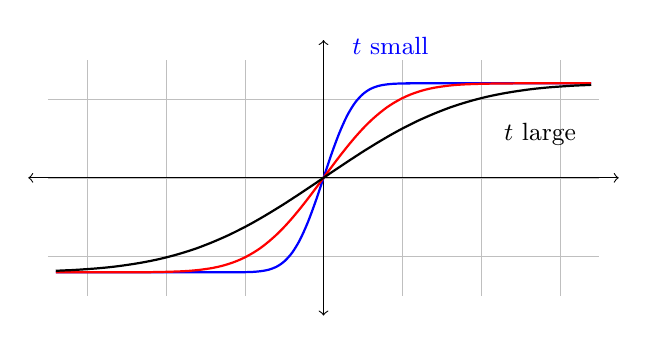
\begin{tikzpicture}
    \draw[ultra thin,color=lightgray] (-3.5,-1.5) grid (3.5,1.5);
    \draw[<->] (-3.75,0) -- (3.75,0);
    \draw[<->] (0,-1.75) -- (0,1.75);
    \draw [thick, smooth, color=blue] plot coordinates {(-3.40,-1.200) (-1.20,-1.200) (-1.10,-1.199) (-1.00,-1.198) (-0.90,-1.195) (-0.80,-1.186) (-0.70,-1.168) (-0.60,-1.131) (-0.50,-1.063) (-0.40,-0.953) (-0.30,-0.789) (-0.20,-0.567) (-0.10,-0.298) (0.00,0.000) (0.10,0.298) (0.20,0.567) (0.30,0.789) (0.40,0.953) (0.50,1.063) (0.60,1.131) (0.70,1.168) (0.80,1.186) (0.90,1.195) (1.00,1.198) (1.10,1.199) (1.20,1.200) (3.40,1.200)};
    \draw [thick, smooth, color=red] plot coordinates {(-3.40,-1.200) (-2.50,-1.200) (-2.40,-1.199) (-2.30,-1.199) (-2.20,-1.198) (-2.10,-1.196) (-2.00,-1.194) (-1.90,-1.191) (-1.80,-1.187) (-1.70,-1.181) (-1.60,-1.172) (-1.50,-1.159) (-1.40,-1.143) (-1.30,-1.121) (-1.20,-1.092) (-1.10,-1.056) (-1.00,-1.011) (-0.90,-0.956) (-0.80,-0.891) (-0.70,-0.813) (-0.60,-0.725) (-0.50,-0.625) (-0.40,-0.514) (-0.30,-0.394) (-0.20,-0.267) (-0.10,-0.135) (0.00,0.000) (0.10,0.135) (0.20,0.267) (0.30,0.394) (0.40,0.514) (0.50,0.625) (0.60,0.725) (0.70,0.813) (0.80,0.891) (0.90,0.956) (1.00,1.011) (1.10,1.056) (1.20,1.092) (1.30,1.121) (1.40,1.143) (1.50,1.159) (1.60,1.172) (1.70,1.181) (1.80,1.187) (1.90,1.191) (2.00,1.194) (2.10,1.196) (2.20,1.198) (2.30,1.199) (2.40,1.199) (2.50,1.200) (3.40,1.200)};
    \draw [thick, smooth, color=black] plot coordinates {(-3.40,-1.181) (-3.30,-1.176) (-3.20,-1.172) (-3.10,-1.166) (-3.00,-1.159) (-2.90,-1.152) (-2.80,-1.143) (-2.70,-1.133) (-2.60,-1.121) (-2.50,-1.107) (-2.40,-1.092) (-2.30,-1.075) (-2.20,-1.056) (-2.10,-1.035) (-2.00,-1.011) (-1.90,-0.985) (-1.80,-0.956) (-1.70,-0.925) (-1.60,-0.891) (-1.50,-0.853) (-1.40,-0.813) (-1.30,-0.770) (-1.20,-0.725) (-1.10,-0.676) (-1.00,-0.625) (-0.90,-0.571) (-0.80,-0.514) (-0.70,-0.455) (-0.60,-0.394) (-0.50,-0.332) (-0.40,-0.267) (-0.30,-0.202) (-0.20,-0.135) (-0.10,-0.068) (0.00,0.000) (0.10,0.068) (0.20,0.135) (0.30,0.202) (0.40,0.267) (0.50,0.332) (0.60,0.394) (0.70,0.455) (0.80,0.514) (0.90,0.571) (1.00,0.625) (1.10,0.676) (1.20,0.725) (1.30,0.770) (1.40,0.813) (1.50,0.853) (1.60,0.891) (1.70,0.925) (1.80,0.956) (1.90,0.985) (2.00,1.011) (2.10,1.035) (2.20,1.056) (2.30,1.075) (2.40,1.092) (2.50,1.107) (2.60,1.121) (2.70,1.133) (2.80,1.143) (2.90,1.152) (3.00,1.159) (3.10,1.166) (3.20,1.172) (3.30,1.176) (3.40,1.181)};
    \node[color=blue] at (0.85, 1.68) {\small $t$ small};
    \node[color=black] at (2.75, 0.55) {\small $t$ large};
\end{tikzpicture}
\end{center}

Notice that at any $t > 0$, no matter how small, the solution is perfectly smooth and is nonzero at every $x$. Diffusion smooths instantly, and (formally) propagates information infinitely fast -- in sharp contrast with the wave equation's strict speed limit $c$.

\subsection{Heat Conduction in a Finite Bar}

Now let's do a full boundary value problem by separation of variables. Take a bar of length $2L$ occupying $-L \leq x \leq L$, with initial temperature a step,
$$
\theta(x, 0) = H(x) = \begin{cases}
    1 &\mbox{if } 0 \leq x \leq L, \\
    0 &\mbox{if } -L \leq x < 0,
\end{cases}
$$
and ends held at fixed temperatures $\theta(L, t) = 1$ and $\theta(-L, t) = 0$.

There's an immediate obstacle: the boundary conditions aren't homogeneous, so our Sturm--Liouville machinery doesn't apply directly. The fix is to subtract off the \vocab{steady state} -- the time-independent solution the bar will relax towards. Steady solutions of the heat equation in one dimension satisfy $\theta_s'' = 0$, so $\theta_s = Ax + B$, and matching the boundary values,
$$
\theta_s(x) = \frac{x + L}{2L}.
$$
Now write $\hat{\theta}(x, t) = \theta(x, t) - \theta_s(x)$. Then $\hat{\theta}$ still satisfies the diffusion equation, but now with \emph{homogeneous} boundary conditions $\hat\theta(\pm L, t) = 0$ and initial condition $\hat\theta(x, 0) = H(x) - \frac{x + L}{2L}$.

Separating variables, $\hat\theta = X(x) T(t)$ gives
$$
X'' = -\lambda X, \quad \dot{T} = -D \lambda T.
$$
The boundary conditions force $\lambda > 0$ as usual. Our initial condition $\hat\theta(x,0)$ is an odd function of $x$ (check this!), so we only need the odd eigenfunctions
$$
X_n(x) = \sin \frac{n \pi x}{L}, \quad \lambda_n = \frac{n^2 \pi^2}{L^2},
$$
and the corresponding temporal solutions are decaying exponentials,
$$
T_n(t) = \exp\left(-\frac{D n^2 \pi^2}{L^2} t\right).
$$
So
$$
\hat\theta(x, t) = \sum_{n = 1}^{\infty} b_n \sin \frac{n \pi x}{L} \exp\left(-\frac{D n^2 \pi^2}{L^2}t\right).
$$
At $t = 0$ this is a Fourier sine series, so
$$
b_n = \frac{2}{L}\int_0^L \left(H(x) - \frac{x + L}{2L}\right)\sin\frac{n \pi x}{L} \dd x
= \frac{2}{L}\int_0^L \frac{1}{2}\sin\frac{n \pi x}{L} \dd x - \frac{2}{L}\int_0^L \frac{x}{2L}\sin\frac{n \pi x}{L} \dd x.
$$
The first integral is half a square wave, contributing $\frac{2}{n \pi}$ for odd $n$ and $0$ for even $n$; the second is half a sawtooth, contributing $-\frac{(-1)^{n+1}}{n \pi}$. Rather pleasingly, in both the odd and even cases the total comes to the same thing:
$$
b_n = \frac{1}{n \pi}.
$$
Hence, restoring the steady state, the temperature of the bar is
$$
\theta(x, t) = \frac{x + L}{2L} + \sum_{n = 1}^{\infty} \frac{1}{n \pi} \sin \frac{n \pi x}{L} \exp\left(-\frac{Dn^2 \pi^2}{L^2} t\right).
$$

There are two things worth noticing here. First, mode $n$ decays at rate $D n^2 \pi^2/L^2$ -- high harmonics die \emph{extremely} fast, so the solution becomes smooth almost immediately and the late-time behaviour is dominated by the steady state plus the slowest mode. Secondly, for early times the series converges slowly, but there the similarity solution $\frac{1}{2}\left(1 + \erf \left(x/2\sqrt{Dt}\right)\right)$ is an excellent approximation, since the step hasn't yet `felt' the boundaries. The two descriptions hand over to each other around $t \sim L^2/D$, the natural diffusion timescale.

\section{Laplace's Equation}

If we look for \emph{steady} states of the wave or diffusion equations -- solutions with no time dependence at all -- both reduce to \vocab{Laplace's equation}
$$
\nabla^2 \phi = 0.
$$
Solutions of Laplace's equation are called \vocab{harmonic functions}. The equation shows up everywhere: steady heat flow, electrostatic and gravitational potentials ($\vv F = -\nabla \phi$), and irrotational incompressible fluid flow ($\vv v = \nabla \phi$).

Laplace's equation is solved on a domain $D$, with data on the boundary $\partial D$ rather than initial conditions. The two standard types are:
\begin{enumerate}[label=(\roman*)]
    \item \vocab{Dirichlet conditions}: $\phi$ specified on $\partial D$;
    \item \vocab{Neumann conditions}: the normal derivative $\partial \phi / \partial n = \hat{\vv n} \cdot \nabla \phi$ specified on $\partial D$.
\end{enumerate}

\subsection{Uniqueness}

Before solving anything, let's establish that boundary data pins the solution down.

\begin{theorem}[Uniqueness for the Dirichlet Problem]
    Suppose $\nabla^2 \phi = 0$ on a bounded domain $D$ with $\phi = f$ given on $\partial D$. Then the solution, if it exists, is unique.
\end{theorem}
\begin{proof}
    Suppose $\phi_1, \phi_2$ are both solutions and let $\psi = \phi_1 - \phi_2$, so that $\nabla^2 \psi = 0$ in $D$ and $\psi = 0$ on $\partial D$.
    Consider
    $$
    \int_D \abs{\nabla \psi}^2 \dd V = \int_D \left[\nabla \cdot (\psi \nabla \psi) - \psi \nabla^2 \psi \right]\dd V = \int_{\partial D} \psi \frac{\partial \psi}{\partial n} \dd S = 0,
    $$
    using the divergence theorem and then both $\nabla^2 \psi = 0$ and $\psi = 0$ on $\partial D$.
    Since $\abs{\nabla \psi}^2 \geq 0$ and integrates to zero, $\nabla \psi \equiv 0$, so $\psi$ is constant on $D$; the boundary condition then forces $\psi \equiv 0$.
\end{proof}

For Neumann conditions the same argument shows the solution is unique \emph{up to an additive constant}, which is the best one could hope for.

The plan for the rest of this section is to run separation of variables in each of the standard coordinate systems -- Cartesian, plane polar, cylindrical and spherical -- and see which special functions each geometry summons.

\subsection{Cartesian Coordinates}

In $\R^3$, Laplace's equation reads $\phi_{xx} + \phi_{yy} + \phi_{zz} = 0$. Seeking $\phi = X(x) Y(y) Z(z)$ and dividing by $XYZ$,
$$
\frac{X''}{X} + \frac{Y''}{Y} + \frac{Z''}{Z} = 0.
$$
Each ratio must be constant, and the three constants sum to zero -- so they can't all have the same sign. If the boundary conditions make $X$ and $Y$ oscillatory, say $X''/X = -\lambda_\ell$ and $Y''/Y = -\lambda_m$ with $\lambda_\ell, \lambda_m > 0$, then necessarily
$$
\frac{Z''}{Z} = \lambda_\ell + \lambda_m > 0,
$$
and $Z$ is a growing/decaying exponential. This is characteristic of Laplace's equation: it cannot oscillate in every direction at once.

\begin{example}[Steady Heat Flow in a Semi-Infinite Bar]
    Consider a bar with rectangular cross-section, occupying $0 \leq x \leq a$, $0 \leq y \leq b$, $z \geq 0$. The four long sides are held at $\phi = 0$, the end $z = 0$ is held at $\phi = 1$, and $\phi \rightarrow 0$ far down the bar as $z \rightarrow \infty$. What is the steady temperature inside?

    \begin{center}
    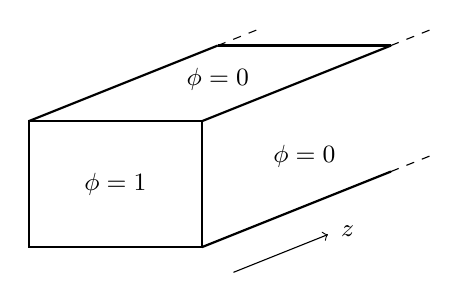
\begin{tikzpicture}
        \draw[thick] (0,0) rectangle (2.2,1.6);
        \draw[thick] (0,1.6) -- (2.4,2.56);
        \draw[thick] (2.2,1.6) -- (4.6,2.56);
        \draw[thick] (2.2,0) -- (4.6,0.96);
        \draw[thick] (2.4,2.56) -- (4.6,2.56);
        \draw[dashed] (4.6,2.56) -- (5.15,2.78);
        \draw[dashed] (4.6,0.96) -- (5.15,1.18);
        \draw[dashed] (2.4,2.56) -- (2.95,2.78);
        \node at (1.1, 0.8) {\small $\phi = 1$};
        \node at (2.4, 2.13) {\small $\phi = 0$};
        \node at (3.5, 1.15) {\small $\phi = 0$};
        \draw[->] (2.6,-0.32) -- (3.8,0.16);
        \node at (4.05,0.2) {\small $z$};
    \end{tikzpicture}
    \end{center}

    The homogeneous conditions $X(0) = X(a) = 0$ and $Y(0) = Y(b) = 0$ give the familiar eigenfunctions
    $$
    X_\ell(x) = \sin \frac{\ell \pi x}{a}, \quad \lambda_\ell = \frac{\ell^2 \pi^2}{a^2}, \qquad Y_m(y) = \sin \frac{m \pi y}{b}, \quad \lambda_m = \frac{m^2 \pi^2}{b^2}.
    $$
    Then $Z'' = (\lambda_\ell + \lambda_m) Z$, and discarding the growing exponential (since $\phi \to 0$ as $z \to \infty$),
    $$
    Z_{\ell m}(z) = \exp\left[-\left(\frac{\ell^2}{a^2} + \frac{m^2}{b^2}\right)^{1/2} \pi z\right].
    $$
    The general solution is
    $$
    \phi = \sum_{\ell, m \geq 1} a_{\ell m} \sin \frac{\ell \pi x}{a} \sin \frac{m \pi y}{b} \exp\left[-\left(\frac{\ell^2}{a^2} + \frac{m^2}{b^2}\right)^{1/2} \pi z \right],
    $$
    and imposing $\phi = 1$ at $z = 0$ is a double Fourier sine series:
    $$
    a_{\ell m} = \left(\frac{2}{a}\int_0^a \sin \frac{\ell \pi x}{a} \dd x \right)\left(\frac{2}{b} \int_0^b \sin \frac{m \pi y}{b} \dd y\right) = \frac{4}{\ell \pi}\cdot \frac{4}{m \pi} = \frac{16}{\pi^2 \ell m}
    $$
    for $\ell, m$ both odd, and $0$ otherwise (each factor is the square wave computation from before).
    Note that far down the bar, the solution is utterly dominated by the $(\ell, m) = (1,1)$ mode: boundary detail at $z = 0$ is exponentially forgotten, with the crudest features persisting longest.
\end{example}

\subsection{Plane Polar Coordinates}

In two dimensions with polar coordinates $(r, \theta)$, Laplace's equation is
$$
\frac{1}{r}\frac{\partial}{\partial r}\left(r \frac{\partial \phi}{\partial r}\right) + \frac{1}{r^2}\frac{\partial^2 \phi}{\partial \theta^2} = 0.
$$
Separating $\phi = R(r) \Theta(\theta)$ gives
$$
\Theta'' + \mu \Theta = 0, \quad r (r R')' - \mu R = 0.
$$
Periodicity of $\Theta$ forces $\mu = m^2$, $m \in \N$, with $\Theta_m = \cos m \theta, \sin m \theta$.

The radial equation this time is \emph{not} Bessel's equation -- there is no second separation constant (compare the wave equation on the disc, where $\lambda$ appeared). It is an equidimensional equation, so we try $R = r^\beta$:
$$
\beta^2 = m^2 \implies \beta = \pm m,
$$
giving $R_m = r^m$ and $r^{-m}$ for $m \geq 1$. For $m = 0$ we get $(rR')' = 0$, so $R' = c/r$ and
$$
R_0 = \text{const}, \ \log r.
$$
The general solution is therefore
$$
\phi(r, \theta) = \frac{a_0}{2} + c_0 \log r + \sum_{m = 1}^{\infty} (a_m \cos m \theta + b_m \sin m \theta) r^m + \sum_{m = 1}^{\infty} (c_m \cos m \theta + d_m \sin m \theta) r^{-m}.
$$
On a domain containing the origin, regularity kills $\log r$ and all the $r^{-m}$; on an exterior domain, boundedness kills the $r^m$ instead.

\begin{example}[A Soap Film on a Distorted Wire]
    Take a circular wire of radius $1$, distorted slightly out of its plane so that its height is $f(\theta)$, and dip it in soap solution. The (small) height $\phi(r, \theta)$ of the resulting film satisfies Laplace's equation on the unit disc with $\phi(1, \theta) = f(\theta)$.

    Regularity at the origin leaves
    $$
    \phi(r, \theta) = \frac{a_0}{2} + \sum_{m = 1}^{\infty}\left(a_m \cos m \theta + b_m \sin m\theta\right) r^m,
    $$
    and at $r = 1$ this is exactly the Fourier series of $f$:
    $$
    a_m = \frac{1}{\pi} \int_0^{2 \pi} f(\theta) \cos m \theta \dd \theta, \quad b_m = \frac{1}{\pi} \int_0^{2\pi} f(\theta) \sin m \theta \dd \theta.
    $$
    The factor $r^m$ means the high harmonics of the wire's wobble decay rapidly towards the centre of the film: near $r = 0$ the film is almost flat at the average height $\frac{1}{2}a_0$. Once again, Laplace's equation smooths.
\end{example}

\subsection{Cylindrical Polar Coordinates}

In cylindrical polars $(r, \theta, z)$,
$$
\frac{1}{r}\frac{\partial}{\partial r}\left(r \frac{\partial \phi}{\partial r}\right) + \frac{1}{r^2}\frac{\partial^2 \phi}{\partial \theta^2} + \frac{\partial^2 \phi}{\partial z^2} = 0.
$$
Separating $\phi = R(r)\Theta(\theta) Z(z)$ gives
$$
\Theta'' = -m^2 \Theta, \quad Z'' = k^2 Z, \quad r(rR')' + (k^2 r^2 - m^2) R = 0.
$$
Now the radial equation \emph{is} Bessel's equation (in the variable $kr$), because the $z$ separation supplies the second constant $k^2$. The bounded-at-the-axis solutions are $R = J_m(kr)$.

If, say, we solve inside a cylinder of radius $a$ with $\phi = 0$ on the curved surface, then $J_m(ka) = 0$ quantises $k = j_{mn}/a$, and the general solution decaying as $z \rightarrow \infty$ is
$$
\phi(r, \theta, z) = \sum_{m = 0}^{\infty}\sum_{n = 1}^{\infty} \left(a_{mn} \cos m \theta + b_{mn} \sin m \theta\right) J_m\left(\frac{j_{mn}}{a} r\right) e^{-j_{mn}z/a},
$$
with coefficients determined from the data on the end $z = 0$ using the orthogonality relation for Bessel functions from before. Structurally this is identical to the Cartesian semi-infinite bar: oscillation across the cross-section, exponential decay along the axis.

\subsection{Spherical Polar Coordinates}

Finally, spherical polars $(r, \theta, \varphi)$, where
$$
\frac{1}{r^2}\frac{\partial}{\partial r}\left(r^2 \frac{\partial \phi}{\partial r}\right) + \frac{1}{r^2 \sin \theta} \frac{\partial}{\partial \theta}\left(\sin \theta \frac{\partial \phi}{\partial \theta}\right) + \frac{1}{r^2 \sin^2 \theta} \frac{\partial^2 \phi}{\partial \varphi^2} = 0.
$$
We will restrict to the \vocab{axisymmetric} case, where $\phi = \phi(r, \theta)$ has no $\varphi$ dependence. Separating $\phi = R(r) \Theta(\theta)$,
$$
(\sin \theta \, \Theta')' + \lambda \sin \theta\, \Theta = 0, \quad (r^2 R')' = \lambda R.
$$
For the angular equation, substitute $x = \cos \theta$ (so $x \in [-1, 1]$, and $\frac{\dd}{\dd \theta} = -\sin\theta \frac{\dd}{\dd x}$):
$$
\frac{\dd}{\dd x}\left[(1 - x^2) \frac{\dd \Theta}{\dd x}\right] + \lambda \Theta = 0.
$$
This is precisely Legendre's equation! Requiring finiteness at the poles $\theta = 0, \pi$ (i.e.\ $x = \pm 1$) gives
$$
\lambda_\ell = \ell (\ell + 1), \quad \Theta_\ell(\theta) = P_\ell(\cos \theta).
$$
So this is where the Legendre polynomials live: they are the natural angular harmonics on the sphere.

The radial equation $(r^2 R')' = \ell(\ell+1) R$ is again equidimensional; trying $R = r^\beta$ gives
$$
\beta(\beta + 1) = \ell (\ell + 1) \implies \beta = \ell \text{ or } -\ell - 1,
$$
so the general axisymmetric harmonic function is
$$
\phi(r, \theta) = \sum_{\ell = 0}^{\infty}\left(a_\ell r^\ell + \frac{b_\ell}{r^{\ell + 1}}\right) P_\ell(\cos \theta).
$$
Interior problems keep only $r^\ell$; exterior problems (with $\phi \rightarrow 0$ at infinity) keep only $r^{-\ell - 1}$.

\begin{example}[Boundary Data on the Unit Sphere]
    Solve $\nabla^2 \phi = 0$ inside the unit sphere with $\phi(1, \theta) = f(\theta)$. Regularity gives $b_\ell = 0$, so writing $f(\theta) = F(\cos\theta)$,
    $$
    F(x) = \sum_{\ell = 0}^{\infty} a_\ell P_\ell(x) \implies a_\ell = \frac{2 \ell + 1}{2}\int_{-1}^{1} F(x) P_\ell(x) \dd x,
    $$
    a Fourier--Legendre series. For instance if $f(\theta) = \cos^2\theta$, then $x^2 = \frac{1}{3}P_0(x) + \frac{2}{3} P_2(x)$, so
    $$
    \phi(r, \theta) = \frac{1}{3} + \frac{2}{3} r^2 P_2(\cos\theta),
    $$
    and no infinite series is needed at all.
\end{example}

\subsubsection*{The Generating Function for Legendre Polynomials}

We can now pay off a debt from Sturm--Liouville theory. Place a unit point charge at the north pole of the unit sphere, $\vv r_0 = (0, 0, 1)$. Its potential at the point with spherical coordinates $(r, \theta)$ is
$$
\Phi = \frac{1}{\abs{\vv r - \vv r_0}} = \frac{1}{\sqrt{r^2 - 2 r \cos \theta + 1}},
$$
expanding $\abs{\vv r - \vv r_0}^2 = r^2 \sin^2 \theta + (r\cos\theta - 1)^2$. Away from the charge this is an axisymmetric harmonic function, regular at the origin, so for $r < 1$ it \emph{must} have an expansion
$$
\frac{1}{\sqrt{r^2 - 2r x + 1}} = \sum_{\ell = 0}^{\infty} a_\ell P_\ell(x)\, r^\ell, \quad x = \cos \theta.
$$
To find the $a_\ell$, look along the axis $x = 1$: the left side is $1/(1 - r) = \sum_\ell r^\ell$, and $P_\ell(1) = 1$, so $a_\ell = 1$ for every $\ell$. Hence
$$
\frac{1}{\sqrt{1 - 2xt + t^2}} = \sum_{\ell = 0}^{\infty} P_\ell(x)\, t^\ell,
$$
which is the generating function quoted earlier. Expanding the potential of a localised charge distribution in powers of $1/r$ using this identity gives the \emph{multipole expansion} of electrostatics: monopole, dipole, quadrupole terms proportional to $P_0, P_1, P_2$ and so on.

\section{The Dirac Delta Function and Distributions}

We have repeatedly hinted that the right way to think about Green's functions is as responses to \emph{point sources}: a unit impulse concentrated at a single point. To make sense of that we need a `function' which is zero everywhere except one point, yet has total integral $1$. No actual function does this, but the idea is far too useful to abandon -- so in this section we develop the object that makes it precise.

\subsection{The Delta Function}

\begin{definition}[Dirac Delta]
    The \vocab{Dirac delta function} $\delta(x - \xi)$ is the generalised function satisfying
    \begin{enumerate}[label=(\roman*)]
        \item $\delta(x - \xi) = 0$ for all $x \neq \xi$;
        \item $\int_{-\infty}^{\infty} \delta(x - \xi) \dd x = 1$.
    \end{enumerate}
    Its defining role is the \vocab{sampling property}: for any $f$ well-behaved near $\xi$,
    $$
    \int_{-\infty}^{\infty} f(x) \delta(x - \xi) \dd x = f(\xi).
    $$
\end{definition}

Strictly, $\delta$ is not a function at all but a \emph{distribution}, and it only really makes sense sitting inside an integral (though we will happily write equations involving $\delta$ outside integrals, with an integral always implied). Physically, $\delta(x - \xi)$ represents a unit point mass, charge, or impulse located at $\xi$.

A good mental model for $\delta$ is as the limit of increasingly tall, thin spikes of unit area. For instance, take the Gaussians
$$
\delta_\epsilon(x) = \frac{1}{\epsilon \sqrt{\pi}} \exp\left(-\frac{x^2}{\epsilon^2}\right),
$$
as $\epsilon \rightarrow 0$:

\begin{center}
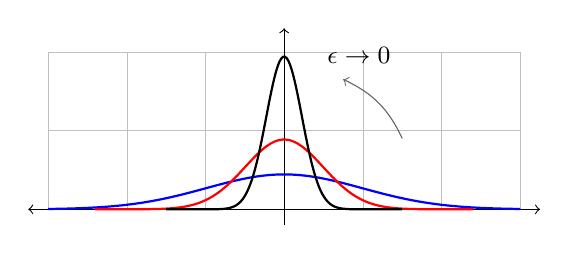
\begin{tikzpicture}
    \draw[ultra thin,color=lightgray] (-3,0) grid (3,2);
    \draw[<->] (-3.25,0) -- (3.25,0);
    \draw[->] (0,-0.2) -- (0,2.3);
    % epsilon = 1.4, 0.7, 0.32  (height 1/(eps sqrt(pi)) scaled by 1.1)
    \draw [thick, samples=100,smooth, color=blue] plot[variable=\t, domain=-3:3] ({\t},{1.1*(1/(1.4*sqrt(pi)))*exp(-\t*\t/(1.4*1.4))});
    \draw [thick, samples=100,smooth, color=red] plot[variable=\t, domain=-2.4:2.4] ({\t},{1.1*(1/(0.7*sqrt(pi)))*exp(-\t*\t/(0.7*0.7))});
    \draw [thick, samples=140,smooth, color=black] plot[variable=\t, domain=-1.5:1.5] ({\t},{1.1*(1/(0.32*sqrt(pi)))*exp(-\t*\t/(0.32*0.32))});
    \node[color=black] at (0.95, 1.95) {\small $\epsilon \to 0$};
    \draw[->, color=black!60] (1.5, 0.9) to[bend right=20] (0.75, 1.65);
\end{tikzpicture}
\end{center}

Let's verify the sampling property for this family. Substituting $y = x/\epsilon$,
\begin{align*}
    \lim_{\epsilon \to 0}\int_{-\infty}^{\infty} \delta_\epsilon(x) f(x) \dd x
    &= \lim_{\epsilon \to 0} \int_{-\infty}^{\infty} \frac{1}{\sqrt{\pi}} e^{-y^2} f(\epsilon y) \dd y \\
    &= \lim_{\epsilon \to 0}\int_{-\infty}^{\infty} \frac{1}{\sqrt{\pi}} e^{-y^2}\left[f(0) + \epsilon y f'(0) + \cdots \right] \dd y = f(0),
\end{align*}
using $\int e^{-y^2} \dd y = \sqrt{\pi}$. The Gaussian family is not special: the \emph{Dirichlet kernel} $\delta_n(x) = \frac{\sin nx}{\pi x}$ and spike families like $\frac{n}{2}\operatorname{sech}^2 (nx)$ work equally well as $n \to \infty$. The limit object is the same $\delta$ in every case.

\subsection{Distributions and Test Functions}

Let's spend a moment making this respectable. The trick is to stop asking for the value of $\delta$ at points, and instead define it by \emph{how it acts on nice functions}.

\begin{definition}[Test Function]
    A \vocab{test function} $\varphi : \R \rightarrow \R$ is a smooth function which vanishes outside some bounded interval.
\end{definition}

\begin{definition}[Distribution]
    A \vocab{distribution} (or \vocab{generalised function}) $T$ is a continuous linear map from test functions to $\R$, written
    $$
    T[\varphi] = \int_{-\infty}^{\infty} T(x) \varphi(x) \dd x,
    $$
    where the integral notation is formal.
\end{definition}

Every ordinary (integrable) function $f$ defines a distribution via $\varphi \mapsto \int f \varphi \dd x$, but there are more distributions than functions: the delta function is the distribution
$$
\delta[\varphi] = \varphi(0),
$$
which is a perfectly well-defined linear map, even though no function represents it.

The real payoff is that distributions can always be differentiated. If $T$ were an honest differentiable function, integration by parts would give $\int T' \varphi \dd x = -\int T \varphi' \dd x$ (the boundary terms vanish since $\varphi$ has bounded support). So we simply \emph{define} the \vocab{distributional derivative} by
$$
T'[\varphi] = -T[\varphi'].
$$
With this definition every distribution is infinitely differentiable, and we can differentiate functions with corners and jumps without guilt.

\begin{example}[Derivative of the Heaviside Function]
    The \vocab{Heaviside step function} is
    $$
    H(x) = \begin{cases}
        1 &\mbox{if } x \geq 0, \\
        0 &\mbox{if } x < 0.
    \end{cases}
    $$
    As a distribution,
    $$
    H'[\varphi] = -H[\varphi'] = -\int_0^{\infty} \varphi'(x) \dd x = \varphi(0) = \delta[\varphi],
    $$
    so $H' = \delta$ in the sense of distributions -- the jump differentiates to a spike. Consistently, $H(x) = \int_{-\infty}^x \delta(t) \dd t$.
\end{example}

\begin{example}[Derivative of the Delta Function]
    Similarly $\delta'$ is defined by
    $$
    \int_{-\infty}^{\infty} \delta'(x - \xi) f(x) \dd x = -\int_{-\infty}^{\infty} \delta(x - \xi) f'(x) \dd x = -f'(\xi),
    $$
    valid whenever $f$ is smooth at $\xi$. One can visualise $\delta'$ as the limit of the derivatives of our Gaussian spikes: a violent up-down pair, which `measures' minus the slope of $f$ at the point.
\end{example}

\subsection{Properties of the Delta Function}

The following properties get used constantly; each is proved by substitution inside an integral against a well-behaved $f$.

\begin{enumerate}[label=(\roman*)]
    \item (Sampling on an interval)
    $$
    \int_a^b f(x) \delta(x - \xi) \dd x = \begin{cases}
        f(\xi) &\mbox{if } a < \xi < b, \\
        0 &\mbox{otherwise}.
    \end{cases}
    $$
    \item (Evenness) $\delta(-(x - \xi)) = \delta(x - \xi)$, by the substitution $u = -(x - \xi)$.
    \item (Scaling) For $a \neq 0$,
    $$
    \delta(a(x - \xi)) = \frac{1}{\abs{a}}\delta(x - \xi).
    $$
    \item (Composition) If $g$ has isolated simple roots $x_1, \dots, x_n$ (so $g'(x_i) \neq 0$), then
    $$
    \delta(g(x)) = \sum_{i = 1}^{n} \frac{\delta(x - x_i)}{\abs{g'(x_i)}},
    $$
    since near each root $g(x) \approx g'(x_i)(x - x_i)$ and we can apply scaling.
    \item (Isolation) If $g$ is continuous at $\xi$ then $g(x) \delta(x - \xi) = g(\xi)\delta(x - \xi)$.
\end{enumerate}

\subsection{Eigenfunction Expansions of the Delta Function}

Here is a question that will matter a lot for Green's functions: what is the Fourier series of $\delta(x)$? Working on $[-L, L]$ with the complex series $\delta(x) = \sum_n c_n e^{i n \pi x/L}$, the coefficients are
$$
c_n = \frac{1}{2L}\int_{-L}^{L} \delta(x) e^{-i n \pi x/L} \dd x = \frac{1}{2L},
$$
all equal! So
$$
\delta(x) = \frac{1}{2L} \sum_{n = -\infty}^{\infty} e^{i n \pi x / L}.
$$
This series diverges wildly at $x = 0$, exactly as it should. It is `equal' to $\delta$ in the distributional sense: integrated against any Fourier-expandable $f$, term-by-term integration gives $f(0)$. Extended periodically, this is a sum of delta spikes at $x = 2mL$ for $m \in \Z$, called the \vocab{Dirac comb}.

More generally, take any Sturm--Liouville system $\{y_n\}$ with weight $w$ on $[a, b]$. Expanding $\delta(x - \xi) = \sum_n a_n y_n(x)$ using the standard coefficient formula,
$$
a_n = \frac{\int_a^b w(x) y_n(x) \delta(x - \xi) \dd x}{\int_a^b w y_n^2 \dd x} = \frac{w(\xi) y_n(\xi)}{N_n}, \quad N_n = \int_a^b w y_n^2 \dd x,
$$
so
$$
\delta(x - \xi) = w(\xi) \sum_{n = 1}^{\infty} \frac{y_n(\xi) y_n(x)}{N_n} = w(x) \sum_{n = 1}^{\infty} \frac{y_n(\xi) y_n(x)}{N_n},
$$
where swapping $w(\xi)$ for $w(x)$ is legitimate by the isolation property. This formula is the \emph{completeness relation} in disguise -- indeed, it's often taken as the definition of completeness of the family $\{y_n\}$.

\begin{example}
    For the sine functions $y_n = \sin n \pi x$ on $[0, 1]$ (so $w = 1$, $N_n = 1/2$),
    $$
    \delta(x - \xi) = 2 \sum_{n = 1}^{\infty} \sin (n \pi \xi) \sin (n \pi x), \quad 0 < \xi < 1.
    $$
\end{example}

\section{Green's Functions for ODEs}

We now come back to the idea we extracted from Sturm--Liouville theory: solving $\mathcal{L} y = f$ by finding an integral kernel $G$ with
$$
y(x) = \int_a^b G(x, \xi) f(\xi) \dd \xi.
$$
Armed with the delta function, we can now say precisely what $G$ is, and construct it directly.

\subsection{Motivation: A Massive String}

Consider a static string with tension $T$ and mass density $\mu$, suspended between fixed ends $y(0) = y(1) = 0$ and sagging under gravity. Balancing forces as in our wave equation derivation (but with no time dependence),
$$
T \frac{\dd^2 y}{\dd x^2} - \mu g = 0, \quad \text{i.e.} \quad -y'' = f, \quad f = -\frac{\mu g}{T}.
$$
We can of course just integrate twice: imposing the boundary conditions gives
$$
y(x) = -\frac{\mu g}{T}\cdot \frac{1}{2}x (1 - x).
$$

But here is a more instructive route. Imagine replacing the continuous string by a very light string carrying a single point mass $\delta m = \mu \, \delta x$ at position $\xi$. The string is then straight on either side of the mass, and resolving forces at the mass point (small angles again) gives the tent-shaped displacement
$$
y(x) = -\frac{\delta m\, g}{T} \times \begin{cases}
    x (1 - \xi) &\mbox{if } x < \xi, \\
    \xi (1 - x) &\mbox{if } x > \xi.
\end{cases}
$$
Now, the equation is linear, so we can superpose: hanging point masses at positions $\xi_1, \xi_2, \dots$ adds the corresponding displacements. Taking the continuum limit, with $f(\xi) \dd \xi$ playing the role of the force from the mass element at $\xi$,
$$
y(x) = \int_0^1 f(\xi)\, G(x, \xi) \dd \xi, \quad \text{where } G(x, \xi) = \begin{cases}
    x(1 - \xi) &\mbox{if } x < \xi, \\
    \xi(1 - x) &\mbox{if } x > \xi
\end{cases}
$$
is the response to a \emph{unit} point force at $\xi$. You can check by direct integration that this reproduces $y = -\frac{\mu g}{2T}x(1 - x)$ exactly. The function $G$ -- the shape of a string plucked by a unit point load -- is the Green's function of the operator $-\dd^2/\dd x^2$ with these boundary conditions.

\subsection{Definition and the Jump Condition}

\begin{definition}[Green's Function]
    Let $\mathcal{L} y = \alpha(x) y'' + \beta(x) y' + \gamma(x) y$ on $a \leq x \leq b$, with $\alpha \neq 0$ and $\alpha, \beta, \gamma$ continuous and bounded, with homogeneous boundary conditions $y(a) = y(b) = 0$. The \vocab{Green's function} of $\mathcal{L}$ is the solution $G(x, \xi)$, satisfying the boundary conditions, of
    $$
    \mathcal{L} G(x, \xi) = \delta(x - \xi).
    $$
\end{definition}

Given the Green's function, the solution of $\mathcal{L}y = f$ is immediate. Setting
$$
y(x) = \int_a^b G(x, \xi) f(\xi) \dd \xi,
$$
we can check
$$
\mathcal{L} y = \int_a^b \mathcal{L}G(x, \xi) f(\xi) \dd \xi = \int_a^b \delta(x - \xi) f(\xi) \dd \xi = f(x),
$$
and $y$ inherits the homogeneous boundary conditions from $G$. So $G$ genuinely is the inverse operator: $\mathcal{L}^{-1} = \int_a^b \dd \xi \, G(x, \xi)$.

What does $G$ look like? Away from $x = \xi$ the delta function vanishes, so $G$ solves the \emph{homogeneous} equation on each side:
$$
G(x, \xi) = \begin{cases}
    G_1(x, \xi) &\mbox{if } a \leq x < \xi, \\
    G_2(x, \xi) &\mbox{if } \xi < x \leq b,
\end{cases}
\quad \mathcal{L}G_1 = \mathcal{L}G_2 = 0,
$$
with $G_1(a, \xi) = 0$ and $G_2(b, \xi) = 0$. It remains to see how the two halves glue at $x = \xi$, and this is where the delta function makes itself felt:
\begin{enumerate}[label=(\roman*)]
    \item \emph{Continuity}: $G_1(\xi, \xi) = G_2(\xi, \xi)$;
    \item \emph{Jump condition}: the derivative jumps by exactly
    $$
    \left[\frac{\partial G}{\partial x}\right]_{\xi_-}^{\xi_+} = \frac{1}{\alpha(\xi)}.
    $$
\end{enumerate}
To see why, integrate $\mathcal{L}G = \delta(x - \xi)$ over a shrinking interval $[\xi - \epsilon, \xi + \epsilon]$. The right side integrates to $1$. On the left, $\int \alpha G'' \dd x \rightarrow \alpha(\xi) [G']^{\xi_+}_{\xi_-}$, while the $\beta G'$ and $\gamma G$ terms contribute nothing in the limit \emph{provided} $G$ is continuous (a jump in $G$ itself would make $G''$ too singular -- a $\delta'$ -- which nothing on the right-hand side could match). Hence the two conditions above.

So the picture to hold in mind: $G(\cdot, \xi)$ is built from homogeneous solutions on either side, tied down at the ends, continuous at $\xi$, with a kink there of size $1/\alpha(\xi)$.

\begin{center}
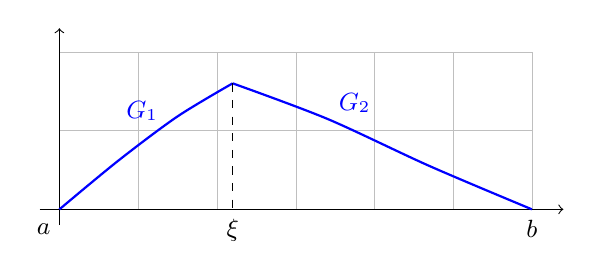
\begin{tikzpicture}
    \draw[ultra thin,color=lightgray] (0,0) grid (6,2);
    \draw[->] (-0.25,0) -- (6.4,0);
    \draw[->] (0,-0.2) -- (0,2.3);
    % kinked Green's function: rises from (0,0) to (2.2,1.6), falls to (6,0), slight curves
    \draw [thick, color=blue] plot [smooth] coordinates {(0,0) (0.75,0.62) (1.5,1.18) (2.2,1.6)};
    \draw [thick, color=blue] plot [smooth] coordinates {(2.2,1.6) (3.4,1.15) (4.7,0.55) (6,0)};
    \draw [dashed] (2.2,1.6) -- (2.2,0) node[below] {\small $\xi$};
    \node at (-0.2,-0.25) {\small $a$};
    \node at (6,-0.25) {\small $b$};
    \node[color=blue] at (1.05, 1.25) {\small $G_1$};
    \node[color=blue] at (3.75, 1.35) {\small $G_2$};
\end{tikzpicture}
\end{center}

\subsection{Explicit Construction}

Let's carry out the construction in general. Let $y_1, y_2$ be independent solutions of $\mathcal{L} y = 0$. Some linear combination $y_-(x)$ satisfies the left boundary condition $y_-(a) = 0$, and some combination $y_+(x)$ satisfies $y_+(b) = 0$. Then
$$
G_1 = C y_-(x), \quad G_2 = D y_+(x),
$$
for constants (in $x$!) $C, D$ which may depend on $\xi$. The gluing conditions read
$$
C y_-(\xi) = D y_+(\xi), \quad D y_+'(\xi) - C y_-'(\xi) = \frac{1}{\alpha(\xi)}.
$$
Solving this pair of linear equations,
$$
C(\xi) = \frac{y_+(\xi)}{\alpha(\xi) W(\xi)}, \quad D(\xi) = \frac{y_-(\xi)}{\alpha(\xi) W(\xi)},
$$
where
$$
W(\xi) = y_-(\xi) y_+'(\xi) - y_+(\xi) y_-'(\xi)
$$
is the \vocab{Wronskian} of $y_-$ and $y_+$, which is nonzero as long as $y_-$ and $y_+$ are independent.\footnote{If $y_-$ and $y_+$ are \emph{not} independent, then there is a nontrivial homogeneous solution satisfying both boundary conditions -- i.e.\ $\lambda = 0$ is an eigenvalue -- and no Green's function exists. Compare trying to invert a singular matrix.} Hence
$$
G(x, \xi) = \begin{cases}
    \dfrac{y_-(x) y_+(\xi)}{\alpha(\xi) W(\xi)} &\mbox{if } a \leq x \leq \xi, \\[2ex]
    \dfrac{y_-(\xi) y_+(x)}{\alpha(\xi) W(\xi)} &\mbox{if } \xi \leq x \leq b,
\end{cases}
$$
and the solution to our boundary value problem is
$$
y(x) = y_+(x) \int_a^x \frac{y_-(\xi) f(\xi)}{\alpha(\xi) W(\xi)} \dd \xi + y_-(x) \int_x^b \frac{y_+(\xi) f(\xi)}{\alpha(\xi) W(\xi)} \dd \xi.
$$
(Note which piece of $G$ applies in which integral: for $\xi < x$ we are to the right of the source, so $G = G_2$.)

A pleasant fact: if $\mathcal{L}$ is in Sturm--Liouville form, then $\beta = \alpha'$, and a quick computation shows $(\alpha W)' = \alpha W' + \alpha' W = 0$ using the ODE -- so $\alpha(\xi) W(\xi)$ is a \emph{constant}, and the Green's function is manifestly symmetric:
$$
G(x, \xi) = G(\xi, x).
$$
This is the analogue of a self-adjoint matrix having a symmetric inverse, and physically it is a reciprocity principle: the response at $x$ to a source at $\xi$ equals the response at $\xi$ to a source at $x$.

\begin{example}
    Let's solve $y'' - y = f(x)$ with $y(0) = y(1) = 0$.
    The homogeneous solutions are $e^{\pm x}$, and the combinations adapted to the boundary conditions are
    $$
    y_-(x) = \sinh x, \quad y_+(x) = \sinh (1 - x).
    $$
    Here $\alpha = 1$ and
    $$
    \alpha W = \sinh x \cdot (-\cosh(1 - x)) - \sinh(1 - x) \cosh x = -\sinh 1,
    $$
    using the addition formula (constant, as promised). So
    $$
    G(x, \xi) = \begin{cases}
        -\dfrac{\sinh x \sinh (1 - \xi)}{\sinh 1} &\mbox{if } 0 \leq x \leq \xi, \\[2ex]
        -\dfrac{\sinh \xi \sinh(1 - x)}{\sinh 1} &\mbox{if } \xi \leq x \leq 1,
    \end{cases}
    $$
    and
    $$
    y(x) = -\frac{\sinh(1 - x)}{\sinh 1}\int_0^x \sinh \xi \, f(\xi) \dd \xi - \frac{\sinh x}{\sinh 1} \int_x^1 \sinh(1 - \xi) f(\xi) \dd \xi.
    $$
\end{example}

If the boundary conditions are \emph{inhomogeneous}, say $y(0) = 0$, $y(1) = 1$, we handle them exactly as in the heat conduction problem: find any homogeneous solution $y_p$ with $\mathcal{L}y_p = 0$ matching the boundary values (here $y_p = \sinh x/\sinh 1$), subtract it off, and solve the resulting homogeneous-boundary problem with the Green's function.

\subsection{Eigenfunction Expansion of the Green's Function}

We derived at the end of Sturm--Liouville theory the formula
$$
G(x, \xi) = \sum_{n = 1}^{\infty} \frac{y_n(x) y_n(\xi)}{\lambda_n N_n}.
$$
Let's re-derive it from our new definition, as a consistency check. Seek $G(x, \xi) = \sum_n A_n y_n(x)$ satisfying $\mathcal{L}G = \delta(x - \xi)$. Then
$$
\mathcal{L}G = \sum_n A_n \lambda_n w(x) y_n(x),
$$
while the delta function has the expansion $\delta(x - \xi) = w(x)\sum_n y_n(\xi) y_n(x)/N_n$ from the last section. Comparing coefficients,
$$
A_n = \frac{y_n(\xi)}{\lambda_n N_n},
$$
which is exactly the earlier formula. Note again that this only makes sense if no $\lambda_n = 0$.

\subsection{Initial Value Problems}

Green's functions work just as well for initial value problems, with one striking new feature. Suppose we want to solve
$$
\mathcal{L}y = f(t), \quad t \geq a, \quad y(a) = y'(a) = 0,
$$
via $G(t, \tau)$ with $\mathcal{L}G = \delta(t - \tau)$ and $G(a, \tau) = G'(a, \tau) = 0$ (derivatives in $t$).

For $t < \tau$: $G_1$ is a homogeneous solution with $G_1(a) = G_1'(a) = 0$. But a homogeneous solution with both initial conditions zero is identically zero (writing $G_1 = A y_1 + B y_2$, the conditions form a linear system whose determinant is the Wronskian of $y_1, y_2$ at $a$, which is nonzero). So
$$
G_1 \equiv 0 \quad \text{for } t < \tau:
$$
nothing happens before the impulse.

For $t > \tau$: continuity forces $G_2(\tau, \tau) = 0$, so $G_2 = D y_+(t)$ where $y_+$ is the homogeneous solution with $y_+(\tau) = 0$, and the jump condition $G_2'(\tau_+) = 1/\alpha(\tau)$ fixes $D = 1/(\alpha(\tau) y_+'(\tau))$. Hence
$$
G(t, \tau) = \begin{cases}
    0 &\mbox{if } t < \tau, \\[0.5ex]
    \dfrac{y_+(t)}{\alpha(\tau) y_+'(\tau)} &\mbox{if } t > \tau,
\end{cases}
$$
and
$$
y(t) = \int_a^t G(t, \tau) f(\tau) \dd \tau.
$$
Note the upper limit: only forcing \emph{before} time $t$ contributes. \vocab{Causality} is built into the structure of the Green's function -- an idea that will return with force when we study signal processing and PDEs.

\begin{example}
    Solve $y'' - y = f(t)$ with $y(0) = y'(0) = 0$.
    For $t > \tau$ we need the homogeneous solution vanishing at $\tau$, namely $y_+ = \sinh(t - \tau)$, and the jump condition gives ($\alpha = 1$, $y_+'(\tau) = \cosh 0 = 1$) coefficient $1$. So
    $$
    y(t) = \int_0^t \sinh(t - \tau) f(\tau) \dd \tau.
    $$
    Compare this with the boundary value problem for the same operator above -- same equation, completely different Green's function. The Green's function belongs to the operator \emph{together with} its boundary conditions.
\end{example}

\begin{remark}[Higher Order Equations]
    Everything generalises to an $n$th order operator $\mathcal{L}$ with leading coefficient $\alpha(x)$: the Green's function is built from homogeneous solutions satisfying the boundary conditions, with $G, G', \dots, G^{(n - 2)}$ all continuous at $x = \xi$ and a jump
    $$
    G^{(n-1)}(\xi_+) - G^{(n - 1)}(\xi_-) = \frac{1}{\alpha(\xi)}
    $$
    in the top derivative.
\end{remark}

\section{Fourier Transforms}

Fourier series decompose periodic functions into harmonics. But plenty of interesting functions -- a solitary pulse, a decaying signal -- are not periodic at all, and live on the whole real line. The \vocab{Fourier transform} is what Fourier series become when the period is sent to infinity: the discrete spectrum of harmonics merges into a continuum.

\subsection{Definition and the Inversion Theorem}

\begin{definition}[Fourier Transform]
    The \vocab{Fourier transform} of $f(x)$ is
    $$
    \tilde{f}(k) = \FF[f](k) = \int_{-\infty}^{\infty} f(x) e^{-ikx} \dd x,
    $$
    and the \vocab{inverse Fourier transform} is
    $$
    f(x) = \FF^{-1}[\tilde f](x) = \frac{1}{2\pi} \int_{-\infty}^{\infty} \tilde{f}(k) e^{ikx} \dd k.
    $$
\end{definition}

(Beware: other books scatter the $2\pi$ differently -- some split it symmetrically as $1/\sqrt{2\pi}$ on each -- and any internally consistent convention is fine.)

\begin{theorem}[Fourier Inversion Theorem]
    If $f$ and $\tilde f$ are absolutely integrable, then
    $$
    \FF^{-1}\big[\FF[f]\big](x) = f(x)
    $$
    at all points where $f$ is continuous; at a jump the right-hand side gives $\frac{1}{2}(f(x_+) + f(x_-))$, just as for Fourier series.
\end{theorem}

Rather than prove this, let's see why it's plausible by deriving the transform as a limit of Fourier series. Take $f$ on $[-L, L]$ with complex Fourier series
$$
f(x) = \sum_{n = -\infty}^{\infty} c_n e^{i k_n x}, \quad k_n = \frac{n \pi}{L},
$$
and write $\Delta k = \pi/L$ for the spacing of the wavenumbers. Then
$$
c_n = \frac{1}{2L}\int_{-L}^{L} f(u) e^{-i k_n u} \dd u = \frac{\Delta k}{2 \pi} \int_{-L}^L f(u) e^{-i k_n u} \dd u,
$$
so
$$
f(x) = \sum_{n = -\infty}^{\infty} \frac{\Delta k}{2 \pi} e^{i k_n x} \int_{-L}^{L} f(u) e^{-i k_n u} \dd u.
$$
As $L \rightarrow \infty$, $\Delta k \rightarrow 0$, and the sum over $n$ is a Riemann sum for an integral over $k$:
$$
f(x) \rightarrow \frac{1}{2 \pi}\int_{-\infty}^{\infty} e^{ikx}\left(\int_{-\infty}^{\infty} f(u) e^{-iku} \dd u\right) \dd k = \FF^{-1}\big[\FF [f]\big](x).
$$

\begin{example}[The Gaussian]
    Let $f(x) = \frac{1}{\sigma \sqrt{\pi}} e^{-x^2/\sigma^2}$. Since $\sin kx$ is odd, only the cosine part survives:
    $$
    \tilde{f}(k) = \frac{1}{\sigma \sqrt{\pi}}\int_{-\infty}^{\infty} e^{-x^2/\sigma^2} \cos (kx) \dd x.
    $$
    Differentiating under the integral sign and integrating by parts,
    $$
    \frac{\dd \tilde f}{\dd k} = \frac{-1}{\sigma \sqrt{\pi}} \int_{-\infty}^{\infty} x e^{-x^2/\sigma^2} \sin(kx) \dd x = -\frac{k \sigma^2}{2} \tilde{f}(k).
    $$
    This little ODE gives $\tilde{f}(k) = C e^{-k^2 \sigma^2/4}$, and setting $k = 0$ (where the integral is just the total area, $1$) gives $C = 1$:
    $$
    \tilde{f}(k) = e^{-k^2 \sigma^2 / 4}.
    $$
    So the transform of a Gaussian is another Gaussian, with \emph{inverted} width: a narrow pulse has a broad spectrum and vice versa. (Readers who have met quantum mechanics will recognise the germ of the uncertainty principle.)
\end{example}

\subsection{Properties of the Fourier Transform}

The Fourier transform converts awkward operations into easy ones. Throughout, $\tilde{f} = \FF[f]$.
\begin{enumerate}[label=(\roman*)]
    \item (Linearity) $\FF[\lambda f + \mu g] = \lambda \tilde f + \mu \tilde g$.
    \item (Translation) $\FF[f(x - \lambda)](k) = e^{-i \lambda k} \tilde{f}(k)$.
    \item (Frequency shift) $\FF[e^{i \lambda x} f(x)](k) = \tilde{f}(k - \lambda)$.
    \item (Scaling) $\FF[f(\lambda x)](k) = \frac{1}{\abs{\lambda}} \tilde{f}(k/\lambda)$.
    \item (Multiplication by $x$) $\FF[x f(x)](k) = i \tilde{f}'(k)$.
    \item (Differentiation) $\FF[f'(x)](k) = ik \tilde{f}(k)$.
\end{enumerate}
Each is a one-line substitution or integration by parts; let's do the most important, (vi):
$$
\int_{-\infty}^{\infty} f'(x) e^{-ikx}\dd x = \Big[f(x) e^{-ikx}\Big]_{-\infty}^{\infty} + ik \int_{-\infty}^{\infty} f(x) e^{-ikx} \dd x = i k \tilde{f}(k),
$$
where the boundary term dies since $f \to 0$ at infinity (a consequence of absolute integrability). \emph{Differentiation becomes multiplication by $ik$} -- this single fact is why Fourier transforms solve differential equations.

There is also a pleasing \vocab{duality}: the inversion formula says $f(-x) = \frac{1}{2\pi}\int \tilde f(k) e^{-ikx} \dd k$, which upon relabelling $x \leftrightarrow k$ reads
$$
\FF\big[\tilde{f}\,\big](k) = 2 \pi f(-k).
$$
Transforming four times gets you home: $\FF^4[f] = 4\pi^2 f$. In practice duality lets every transform we compute do double duty.

\begin{example}[The Top Hat and sinc]
    Let $f$ be the `top hat'
    $$
    f(x) = \begin{cases}
        1 &\mbox{if } \abs{x} \leq a, \\
        0 &\mbox{otherwise}.
    \end{cases}
    $$
    Then
    $$
    \tilde{f}(k) = \int_{-a}^{a} e^{-ikx} \dd x = \int_{-a}^a \cos (kx) \dd x = \frac{2 \sin ka}{k},
    $$
    a scaled \emph{sinc} function.

    \begin{center}
    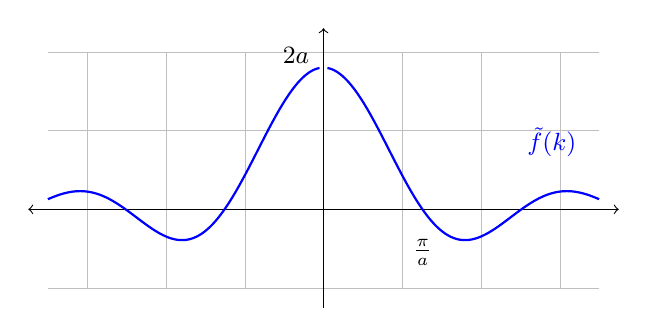
\begin{tikzpicture}
        \draw[ultra thin,color=lightgray] (-3.5,-1) grid (3.5,2);
        \draw[<->] (-3.75,0) -- (3.75,0);
        \draw[->] (0,-1.25) -- (0,2.3);
        % 2 sin(ka)/k with a = 2.5 (k in figure units), y scaled by 0.36: peak 2a*0.36 = 1.8
        \draw [thick, samples=250,smooth, color=blue] plot[variable=\t, domain=-3.5:-0.05] ({\t},{0.72*sin(deg(2.5*\t))/\t});
        \draw [thick, samples=250,smooth, color=blue] plot[variable=\t, domain=0.05:3.5] ({\t},{0.72*sin(deg(2.5*\t))/\t});
        \node at (-0.35, 1.95) {\small $2a$};
        \node at (1.26, -0.55) {\small $\frac{\pi}{a}$};
        \node[color=blue] at (2.9, 0.85) {\small $\tilde{f}(k)$};
    \end{tikzpicture}
    \end{center}

    Notice that $f$ has bounded support but $\tilde f$ spreads over all $k$, decaying only like $1/k$ -- the slow decay is the price of the sharp edges. As a bonus, applying the inversion theorem at $x = 0$ (where $f$ is continuous, $f(0) = 1$) gives
    $$
    1 = \frac{1}{2\pi}\int_{-\infty}^{\infty} \frac{2 \sin ka}{k} \dd k,
    $$
    from which (relabelling and using evenness) we obtain the \vocab{Dirichlet discontinuous formula}
    $$
    \int_0^{\infty} \frac{\sin a x}{x} \dd x = \frac{\pi}{2}\sgn a = \begin{cases}
        \pi/2 &\mbox{if } a > 0, \\
        0 &\mbox{if } a = 0, \\
        -\pi/2 &\mbox{if } a < 0.
    \end{cases}
    $$
\end{example}

\subsection{Convolution and Parseval's Theorem}

Multiplication of transforms corresponds to a mixing operation on the original functions.

\begin{definition}[Convolution]
    The \vocab{convolution} of $f$ and $g$ is
    $$
    (f * g)(x) = \int_{-\infty}^{\infty} f(y) g(x - y) \dd y.
    $$
\end{definition}

\begin{theorem}[Convolution Theorem]
    $\FF[f * g] = \tilde{f}(k)\, \tilde{g}(k)$. Dually, $\FF[fg] = \frac{1}{2\pi} \big(\tilde{f} * \tilde{g}\big)$.
\end{theorem}
\begin{proof}
    Start from the product and invert:
    \begin{align*}
        \FF^{-1}\big[\tilde f \tilde g\big](x) &= \frac{1}{2\pi}\int_{-\infty}^{\infty} \tilde{f}(k) \tilde{g}(k) e^{ikx} \dd k \\
        &= \frac{1}{2\pi}\int_{-\infty}^{\infty} \left(\int_{-\infty}^{\infty} f(y) e^{-iky} \dd y\right) \tilde{g}(k) e^{ikx} \dd k \\
        &= \int_{-\infty}^{\infty} f(y) \left(\frac{1}{2 \pi}\int_{-\infty}^{\infty} \tilde{g}(k) e^{ik(x - y)} \dd k\right) \dd y \\
        &= \int_{-\infty}^{\infty} f(y)\, g(x - y) \dd y = (f * g)(x). \qedhere
    \end{align*}
\end{proof}

\begin{theorem}[Parseval's Theorem for Fourier Transforms]
    $$
    \int_{-\infty}^{\infty} \abs{f(x)}^2 \dd x = \frac{1}{2\pi} \int_{-\infty}^{\infty} \abs{\tilde{f}(k)}^2 \dd k.
    $$
\end{theorem}
\begin{proof}
    First note that if $h(x) = g^*(-x)$ then $\tilde{h}(k) = \tilde{g}^*(k)$ (substitute and conjugate). Applying the convolution theorem to $f$ and $g^*(-\cdot)$ and evaluating at $x = 0$,
    $$
    \int_{-\infty}^{\infty} f(y)\, g^*(y) \dd y = \frac{1}{2\pi}\int_{-\infty}^{\infty} \tilde{f}(k) \tilde{g}^*(k) \dd k,
    $$
    which says the Fourier transform preserves inner products up to the factor $2\pi$: $\langle g, f\rangle = \frac{1}{2\pi}\langle \tilde{g}, \tilde{f} \rangle$. Taking $g = f$ gives the result.
\end{proof}

\subsection{Fourier Transforms of Generalised Functions}

The class of functions with honest Fourier transforms is a bit restrictive ($f \to 0$ at infinity, etc.), but distributions let us transform far more. The key identity comes from writing out the inversion theorem in full:
$$
f(x) = \frac{1}{2\pi} \int_{-\infty}^{\infty} \left(\int_{-\infty}^{\infty} f(u) e^{-iku} \dd u \right) e^{ikx} \dd k = \int_{-\infty}^{\infty} f(u) \left[\frac{1}{2\pi} \int_{-\infty}^{\infty} e^{ik(x - u)} \dd k\right] \dd u.
$$
For this to spit out $f(x)$ for every $f$, the bracket must be precisely a delta function:
$$
\delta(x - u) = \frac{1}{2\pi}\int_{-\infty}^{\infty} e^{ik(x - u)} \dd k.
$$
This wildly divergent-looking integral is a perfectly good distributional statement, and it immediately gives a dictionary:
\begin{enumerate}[label=(\roman*)]
    \item $\FF[\delta(x)] = 1$, and more generally $\FF[\delta(x - a)] = e^{-ika}$;
    \item $\FF[1] = 2 \pi \delta(k)$ (an infinitely spread function has an infinitely concentrated spectrum);
    \item $\FF[\cos \omega x] = \pi \left(\delta(k - \omega) + \delta(k + \omega)\right)$ and $\FF[\sin \omega x] = i\pi\left(\delta(k + \omega) - \delta(k - \omega)\right)$ -- a pure tone has a spectrum concentrated at $\pm$ its frequency;
    \item from the Dirichlet discontinuous formula, $\FF\left[\frac{1}{2}\sgn x \right] = \frac{1}{ik}$;
    \item for the Heaviside function, writing $H(x) = \frac{1}{2} + \frac{1}{2}\sgn x$,
    $$
    \FF[H](k) = \pi \delta(k) + \frac{1}{ik}.
    $$
\end{enumerate}
As a sanity check on (v): $H' = \delta$ requires $ik \tilde{H} = 1$, which holds since $k \delta(k) = 0$; and $H(x) + H(-x) = 1$ requires $\tilde H(k) + \tilde H(-k) = 2\pi \delta(k)$, which also checks out. Neither condition alone pins $\tilde H$ down -- together they do.

\subsection{Solving Differential Equations with Fourier Transforms}

Here's the general scheme: transform the equation (derivatives become multiplications), solve \emph{algebraically}, and transform back (usually via the convolution theorem).

\begin{example}[A Boundary Value Problem on the Line]
    Solve $y'' - y = f(x)$ with $y \to 0$ as $x \to \pm\infty$. Transforming,
    $$
    (ik)^2 \tilde{y} - \tilde{y} = \tilde{f} \implies \tilde{y}(k) = \frac{-\tilde{f}(k)}{1 + k^2} = \tilde{f}(k)\, \tilde{g}(k), \quad \tilde{g}(k) = \frac{-1}{1 + k^2}.
    $$
    One can check (by computing the transform of $e^{-\abs{x}}$) that $\tilde{g}$ is the transform of $g(x) = -\frac{1}{2}e^{-\abs{x}}$. So by the convolution theorem,
    $$
    y(x) = (f * g)(x) = -\frac{1}{2}\int_{-\infty}^{\infty} f(u) e^{-\abs{x - u}} \dd u.
    $$
    This is exactly a Green's function solution, with $G(x, u) = -\frac{1}{2}e^{-\abs{x - u}}$ -- which is just what we would have built with jump conditions, with the boundary conditions now imposed at $\pm \infty$. The Fourier transform found it for us automatically.
\end{example}

\subsection{Signal Processing and Transfer Functions}

A common situation: a physical system (an amplifier, a suspension bridge, a circuit) receives an input signal $\mathcal{I}(t)$ and produces an output $\mathcal{O}(t)$, with the relationship linear and time-invariant. In the frequency domain such a system can only do one thing: multiply each frequency component by a fixed complex number. That is,
$$
\tilde{\mathcal{O}}(\omega) = \tilde{\mathcal{R}}(\omega)\, \tilde{\mathcal{I}}(\omega),
$$
where $\tilde{\mathcal{R}}(\omega)$ is the \vocab{transfer function} of the system. Its inverse transform $\mathcal{R}(t)$ is the \vocab{response function}, and by the convolution theorem
$$
\mathcal{O}(t) = \int_{-\infty}^{\infty} \mathcal{I}(u)\, \mathcal{R}(t - u) \dd u.
$$
The response function is the output produced by a delta-function kick at $t = 0$ -- it is a Green's function by another name. For a physically realisable system, \emph{causality} demands $\mathcal{R}(t) = 0$ for $t < 0$ (no output before the input), so if the input starts at $t = 0$,
$$
\mathcal{O}(t) = \int_0^t \mathcal{I}(u)\, \mathcal{R}(t - u) \dd u,
$$
which has precisely the shape of our initial value problem Green's function solutions.

Suppose the system is governed by an ODE,
$$
\mathcal{L} \mathcal{O}(t) = \left(a_n \frac{\dd^n}{\dd t^n} + \cdots + a_1 \frac{\dd}{\dd t} + a_0\right)\mathcal{O}(t) = \mathcal{I}(t).
$$
Transforming, each derivative becomes $i \omega$, so
$$
\tilde{\mathcal{R}}(\omega) = \frac{1}{a_0 + a_1 (i\omega) + \cdots + a_n (i \omega)^n}.
$$
To invert, factor the denominator over its roots and expand in partial fractions:
$$
\tilde{\mathcal{R}}(\omega) = \sum_{j = 1}^{J} \sum_{m = 1}^{k_j} \frac{\Gamma_{jm}}{(i \omega - c_j)^m}.
$$
The basic inverse transform (computable directly, for $\re c < 0$) is
$$
\FF^{-1}\left[\frac{1}{i\omega - c}\right](t) = \begin{cases}
    e^{ct} &\mbox{if } t > 0, \\
    0 &\mbox{if } t < 0,
\end{cases}
$$
and repeatedly applying the `multiplication by $t$' rule gives
$$
\FF^{-1}\left[\frac{1}{(i \omega - c)^m}\right](t) = \frac{t^{m - 1}}{(m-1)!} e^{ct} \quad (t > 0).
$$
So provided all roots satisfy $\re c_j < 0$ (a \emph{stable} system -- no exponentially growing responses), the response function is
$$
\mathcal{R}(t) = \sum_{j = 1}^{J}\sum_{m = 1}^{k_j} \Gamma_{jm} \frac{t^{m - 1}}{(m - 1)!} e^{c_j t} \quad \text{for } t > 0,
$$
and zero for $t < 0$. Causality has appeared automatically.

\begin{example}[The Damped Oscillator]
    Consider $y'' + 2p y' + (p^2 + q^2) y = f(t)$ with $p > 0$ and $y(0) = y'(0) = 0$. The transfer function is
    $$
    \tilde{\mathcal{R}}(\omega) = \frac{1}{(i\omega)^2 + 2p (i \omega) + p^2 + q^2} = \frac{1}{(i \omega + p)^2 + q^2},
    $$
    with roots $i \omega = -p \pm iq$, both with negative real part. Partial fractions and the table above give
    $$
    \mathcal{R}(t) = \frac{1}{q} e^{-pt} \sin (qt) \quad (t > 0),
    $$
    a decaying oscillation, and the solution is
    $$
    y(t) = \frac{1}{q}\int_0^t e^{-p(t - \tau)} \sin\big(q(t - \tau)\big) f(\tau) \dd \tau.
    $$
    One can verify directly that $\mathcal{R}(t - \tau)$ satisfies $\mathcal{L}\mathcal{R} = \delta(t - \tau)$: it is the initial-value Green's function of the damped oscillator.
\end{example}

\subsection{Discrete Sampling and the Nyquist Frequency}

In the real world we don't measure signals continuously; we \emph{sample} them, at times $t_n = n \Delta$ for some fixed time step $\Delta$. How much do we lose?

The natural frequency scale is the \vocab{Nyquist frequency}
$$
f_c = \frac{1}{2 \Delta},
$$
the highest frequency the sampling can resolve -- one sample per half-period. Consider sampling a pure tone $g_f(t) = A\cos(2 \pi f t + \varphi)$.
If $f = f_c$ exactly, then
$$
g_{f_c}(t_n) = A \cos (\pi n + \varphi) = A \cos (\varphi) \cos(\pi n),
$$
so the samples only see the combination $A \cos \varphi$: amplitude and phase have become degenerate, and half the information is gone.
Worse, for a frequency \emph{above} Nyquist, $f = f_c + \delta f$, the samples satisfy
$$
g_{f_c + \delta f}(t_n) = g_{f_c - \delta f}(t_n) \quad \text{(up to phase)},
$$
so the high frequency masquerades as the lower frequency $f_c - \delta f$. This is called \vocab{aliasing}, and it's why car wheels appear to spin backwards on film.

If, however, the signal contains \emph{no} frequencies above some $\omega_{\max}$ (it is \vocab{bandwidth-limited}), sampling loses nothing at all:

\begin{theorem}[Nyquist--Shannon Sampling Theorem]
    Let $g$ be bandwidth-limited with $\tilde{g}(\omega) = 0$ for $\abs{\omega} > \omega_{\max}$, and sample at the Nyquist rate, $\Delta = \pi / \omega_{\max}$, giving samples $g_n = g(n \Delta)$. Then $g$ is \emph{exactly} reconstructible:
    $$
    g(t) = \sum_{n = -\infty}^{\infty} g_n \, \frac{\sin (\omega_{\max}t - n \pi)}{\omega_{\max} t - n \pi}.
    $$
\end{theorem}
\begin{proof}
    Since $\tilde{g}$ is supported on the bounded interval $[-\omega_{\max}, \omega_{\max}]$, we can expand it there in a \emph{Fourier series} (in $\omega$!):
    the coefficients of that series are, up to constants, exactly the samples $g_n$, since
    $$
    g_n = \frac{1}{2\pi}\int_{-\omega_{\max}}^{\omega_{\max}} \tilde{g}(\omega) e^{i \pi n \omega/\omega_{\max}} \dd \omega.
    $$
    So the samples determine the periodic extension $\tilde{g}_{\text{per}}(\omega) = \frac{\pi}{\omega_{\max}} \sum_n g_n e^{-i \pi n \omega/\omega_{\max}}$, and multiplying by the top hat on $[-\omega_{\max}, \omega_{\max}]$ recovers $\tilde{g}$ exactly. Inverting,
    $$
    g(t) = \frac{1}{2 \omega_{\max}} \sum_{n = -\infty}^{\infty} g_n \int_{-\omega_{\max}}^{\omega_{\max}} e^{i \omega(t - n \pi/\omega_{\max})} \dd \omega,
    $$
    and each integral is a sinc, giving the stated formula.
\end{proof}

The sinc functions are doing interpolation duty: the $n$th term equals $g_n$ at $t = t_n$ and vanishes at every other sample point.

\subsection{The Discrete Fourier Transform}

Finally, suppose we have only finitely many samples $h_m = h(t_m)$, $t_m = m \Delta$, $m = 0, \dots, N - 1$. We estimate the Fourier transform at the $N$ frequencies $f_n = \frac{n}{N \Delta}$ (which, thanks to aliasing, is the honest number of distinct frequencies available):
$$
\tilde{h}(f_n) = \int_{-\infty}^{\infty} h(t) e^{-2 \pi i f_n t} \dd t \approx \Delta \sum_{m = 0}^{N - 1} h_m e^{-2 \pi i m n /N} = \Delta \,\tilde{h}_n.
$$

\begin{definition}[Discrete Fourier Transform]
    The \vocab{discrete Fourier transform} of the vector $(h_0, \dots, h_{N-1})$ is
    $$
    \tilde{h}_n = \sum_{m = 0}^{N - 1} h_m \, \omega^{mn}, \quad \omega = e^{-2\pi i /N},
    $$
    i.e.\ $\tilde{h} = [\mathrm{DFT}]\, h$ where $[\mathrm{DFT}]_{nm} = \omega^{nm}$ is an $N \times N$ matrix of roots of unity.
\end{definition}

The DFT matrix is (up to scaling) unitary: $[\mathrm{DFT}]^{-1} = \frac{1}{N}[\mathrm{DFT}]^{\dagger}$, so inversion is
$$
h_m = \frac{1}{N} \sum_{n = 0}^{N - 1} \tilde{h}_n e^{2 \pi i mn/N}.
$$
For example, with $N = 4$ we have $\omega = -i$ and
$$
[\mathrm{DFT}] = \begin{pmatrix}
    1 & 1 & 1 & 1 \\
    1 & -i & -1 & i \\
    1 & -1 & 1 & -1 \\
    1 & i & -1 & -i
\end{pmatrix}.
$$
The discrete analogues of our earlier theorems hold, e.g.\ Parseval becomes $\sum_m \abs{h_m}^2 = \frac{1}{N}\sum_n |\tilde{h}_n|^2$, and convolution (defined cyclically) again maps to multiplication.

\begin{remark}[The Fast Fourier Transform]
    Computing the DFT naively costs $O(N^2)$ operations. The \emph{fast Fourier transform} does it in $O(N \log N)$, by splitting the sum into even and odd samples: since $\omega_N^2 = \omega_{N/2}$,
    $$
    \tilde{h}_k = \sum_{m = 0}^{N/2 - 1} h_{2m}\, \omega_{N/2}^{mk} + \omega_N^{k}\sum_{m = 0}^{N/2 - 1} h_{2m + 1}\, \omega_{N/2}^{mk},
    $$
    two DFTs of half the size, and recursing. This algorithm (this material is non-examinable, but too good to omit) is quietly running inside essentially every piece of modern signal-processing equipment.
\end{remark}

\section{The Method of Characteristics}

We now step back and develop a more geometric way of thinking about PDEs, which explains -- among other things -- where d'Alembert's solution really came from, and why the wave, diffusion and Laplace equations behave so differently.

\subsection{Well-Posed Cauchy Problems}

A \vocab{Cauchy problem} consists of a PDE for some function $\phi$ together with auxiliary data (values of $\phi$ and/or its derivatives) specified on some surface -- in two dimensions, a curve. The data is called \vocab{Cauchy data}.
Following Hadamard, we say the problem is \vocab{well-posed} if
\begin{enumerate}[label=(\roman*)]
    \item a solution exists (we haven't demanded too much),
    \item the solution is unique (we haven't demanded too little), and
    \item the solution depends continuously on the data (small measurement errors don't explode).
\end{enumerate}
Which kinds of data make a problem well-posed depends dramatically on the equation: initial data suits the wave and diffusion equations, boundary data suits Laplace's equation, and mixing these up goes badly wrong. The method of characteristics is the tool that explains why.

\subsection{Characteristics of First Order PDEs}

Consider a curve $C$ in the plane, parametrised as $(x(s), y(s))$, with tangent vector $\vv u = (\dd x/\dd s, \dd y/\dd s)$. The derivative of a function $\phi$ along the curve is
$$
\left.\frac{\dd \phi}{\dd s}\right|_C = \frac{\dd x}{\dd s} \frac{\partial \phi}{\partial x} + \frac{\dd y}{\dd s}\frac{\partial \phi}{\partial y} = \vv u \cdot \nabla \phi.
$$

Now consider the general homogeneous first order linear PDE
$$
\alpha(x, y) \frac{\partial \phi}{\partial x} + \beta(x, y) \frac{\partial \phi}{\partial y} = 0.
$$
The left-hand side is exactly the directional derivative of $\phi$ along the vector field $\vv u = (\alpha, \beta)$! So the PDE says something beautifully simple: \emph{$\phi$ is constant along the integral curves of $\vv u$}, i.e.\ the curves solving
$$
\frac{\dd x}{\dd s} = \alpha(x, y), \quad \frac{\dd y}{\dd s} = \beta(x, y).
$$
These curves are called the \vocab{characteristic curves} (or just characteristics) of the PDE. Solving a PDE has been reduced to solving a family of ODEs.

To pose a Cauchy problem, we specify $\phi = f(t)$ along some initial curve $B$, parametrised by $t$ as $(x(t), y(t))$, chosen \emph{transverse} to the characteristics (nowhere tangent to them). Each characteristic then picks up its constant value where it crosses $B$, and carries it across the plane: labelling characteristics by their crossing point $t$, with $s$ the parameter along each (set $s = 0$ on $B$), we get coordinates $(s, t)$ in which the solution is simply
$$
\phi(s, t) = f(t).
$$

\begin{center}
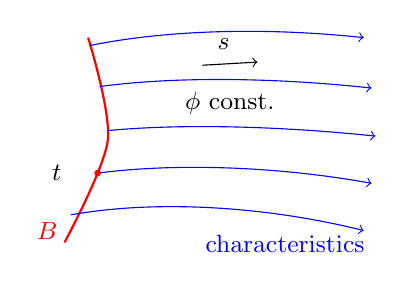
\begin{tikzpicture}
    % initial curve B and fan of characteristics
    \draw[thick, color=red] plot [smooth] coordinates {(-0.4,-1.3) (0.15,0) (-0.1,1.3)};
    \node[color=red] at (-0.62,-1.15) {\small $B$};
    % characteristics crossing B
    \draw[->, color=blue] (-0.32,-0.95) .. controls (0.8,-0.75) and (2.2,-0.85) .. (3.4,-1.15);
    \draw[->, color=blue] (0.02,-0.42) .. controls (1.1,-0.28) and (2.4,-0.35) .. (3.5,-0.55);
    \draw[->, color=blue] (0.15,0.12) .. controls (1.2,0.22) and (2.5,0.16) .. (3.55,0.05);
    \draw[->, color=blue] (0.05,0.68) .. controls (1.1,0.82) and (2.4,0.78) .. (3.5,0.66);
    \draw[->, color=blue] (-0.08,1.2) .. controls (1,1.42) and (2.3,1.42) .. (3.4,1.3);
    \node[color=blue] at (2.4, -1.32) {\small characteristics};
    \node at (1.7, 0.47) {\small $\phi$ const.};
    \fill[color=red] (0.02,-0.42) circle (1.2pt);
    \node at (-0.5, -0.42) {\small $t$};
    \draw[->] (1.35,0.95) -- (2.05,0.99);
    \node at (1.62, 1.22) {\small $s$};
\end{tikzpicture}
\end{center}

Finally, provided the Jacobian $J = x_t y_s - x_s y_t$ of the map $(s,t) \mapsto (x,y)$ is nonzero (this is what transversality buys us), we can invert to find $s(x,y)$, $t(x,y)$ and hence $\phi(x, y) = f(t(x, y))$.

In summary, the recipe is:
\begin{enumerate}
    \item write down the characteristic equations $\dd x/\dd s = \alpha$, $\dd y/\dd s = \beta$;
    \item parametrise the initial curve $B$ by $(x(t), y(t))$;
    \item solve the characteristic equations with initial conditions on $B$ at $s = 0$, obtaining $x(s,t)$, $y(s, t)$;
    \item observe $\phi$ is constant along characteristics, so $\phi(s,t) = f(t)$;
    \item invert to express $(s, t)$ in terms of $(x, y)$.
\end{enumerate}

\begin{example}
    Solve $e^x \phi_x + \phi_y = 0$ with $\phi(x, 0) = \cosh x$.
    The characteristic equations are
    $$
    \frac{\dd x}{\dd s} = e^x, \quad \frac{\dd y}{\dd s} = 1,
    $$
    and the initial curve is $(x, y) = (t, 0)$ at $s = 0$. Solving: $-e^{-x} = s - e^{-t}$ and $y = s$. So along each characteristic, $e^{-x} + y = e^{-t}$, i.e.\ the characteristics are the curves $y = e^{-t} - e^{-x}$, and
    $$
    t = -\log\left(y + e^{-x}\right).
    $$
    Since $\phi$ is constant along characteristics, $\phi(s, t) = \cosh t$, so
    $$
    \phi(x, y) = \cosh \left[\log\left(y + e^{-x}\right)\right] = \frac{1}{2}\left(y + e^{-x} + \frac{1}{y + e^{-x}}\right).
    $$
    One can check directly that this satisfies the PDE and the data.
\end{example}

\subsection{Inhomogeneous First Order PDEs}

Now add a source:
$$
\alpha(x, y) \phi_x + \beta(x, y) \phi_y = \gamma(x, y), \quad \phi = f(t) \text{ on } B.
$$
The characteristics are unchanged, but $\phi$ is no longer constant along them -- instead
$$
\left.\frac{\dd \phi}{\dd s}\right|_C = \gamma\big(x(s), y(s)\big),
$$
an ODE to be solved \emph{along each characteristic}, with initial value $f(t)$ at $s = 0$. The geometry is the same; the data is now transported with modification rather than unchanged.

\begin{example}
    Solve $\phi_x + 2 \phi_y = y e^x$ with $\phi = \sin x$ on the line $y = x$.
    Characteristics: $\dd x/\dd s = 1$, $\dd y /\dd s = 2$, with $(x, y) = (t, t)$ at $s = 0$, giving
    $$
    x = s + t, \quad y = 2s + t.
    $$
    Along a characteristic,
    $$
    \frac{\dd \phi}{\dd s} = y e^x = (2s + t)e^{s + t},
    $$
    and integrating with respect to $s$ (noting $\int 2s e^s \dd s = 2(s-1)e^s$),
    $$
    \phi(s, t) = (2s + t - 2)e^{s + t} + c(t).
    $$
    The initial condition $\phi(0, t) = \sin t$ gives $c(t) = \sin t - (t - 2)e^t$. Inverting $s = y - x$, $t = 2x - y$,
    $$
    \phi(x, y) = (y - 2) e^x + (2 - 2x + y)e^{2x - y} + \sin (2x - y).
    $$
\end{example}

\subsection{Classification of Second Order PDEs}

Let's now bring these ideas to second order equations. The general second order linear PDE in two variables is
$$
a(x,y) \phi_{xx} + 2b(x, y) \phi_{xy} + c(x, y)\phi_{yy} + d \phi_x + e \phi_y + f \phi = 0,
$$
and its behaviour is governed by the \vocab{principal part} -- the top order terms -- encoded in the symmetric matrix
$$
A = \begin{pmatrix}
    a & b \\ b & c
\end{pmatrix}.
$$

\begin{definition}[Classification]
    The PDE is
    \begin{enumerate}[label=(\roman*)]
        \item \vocab{elliptic} if $b^2 - ac < 0$ (eigenvalues of $A$ of the same sign) -- e.g.\ Laplace's equation;
        \item \vocab{hyperbolic} if $b^2 - ac > 0$ (eigenvalues of opposite signs) -- e.g.\ the wave equation;
        \item \vocab{parabolic} if $b^2 - ac = 0$ (a zero eigenvalue) -- e.g.\ the diffusion equation.
    \end{enumerate}
\end{definition}

The terminology comes from the conic sections $a k_1^2 + 2b k_1 k_2 + c k_2^2 = \text{const}$. Note that the classification is pointwise: an equation with variable coefficients can be hyperbolic in one region and elliptic in another.

We say a curve along which $u(x,y)$ is constant is a \vocab{characteristic curve} of the equation if
$$
\begin{pmatrix} u_x & u_y \end{pmatrix} \begin{pmatrix} a & b \\ b & c\end{pmatrix}\begin{pmatrix} u_x \\ u_y\end{pmatrix} = 0.
$$
(For first order equations this reduces to our earlier condition $\vv u \cdot \nabla u = 0$ along characteristics.) Writing the curve as $y = y(x)$ and using $u_x + u_y \frac{\dd y}{\dd x} = 0$ along it, the condition becomes a quadratic for the slope:
$$
a \left(\frac{\dd y}{\dd x}\right)^2 - 2b \frac{\dd y}{\dd x} + c = 0 \implies \frac{\dd y}{\dd x} = \frac{b \pm \sqrt{b^2 - ac}}{a}.
$$
So we can read the classification off geometrically:
\begin{enumerate}[label=(\roman*)]
    \item hyperbolic equations have \emph{two} families of real characteristics;
    \item parabolic equations have exactly one;
    \item elliptic equations have none.
\end{enumerate}
Characteristics are the curves along which information (and discontinuities in derivatives of the solution) propagate. The wave equation moves data along its two families of characteristics; Laplace's equation, with no real characteristics, moves nothing -- its solutions are instantly smooth everywhere, and only boundary data makes sense.

\subsection{Characteristic Coordinates}

For a hyperbolic equation, using the two families of characteristics as a coordinate system $(u, v)$ kills both the $\phi_{uu}$ and $\phi_{vv}$ terms, reducing the equation to \vocab{canonical form}
$$
\frac{\partial^2 \phi}{\partial u \, \partial v} + (\text{lower order terms}) = 0.
$$
(For parabolic equations the canonical form is $\phi_{vv} + \cdots = 0$, and for elliptic ones $\phi_{uu} + \phi_{vv} + \cdots = 0$.)

\begin{example}
    Consider $-y \phi_{xx} + \phi_{yy} = 0$. Here $a = -y$, $b = 0$, $c = 1$, so $b^2 - ac = y$: the equation is hyperbolic for $y > 0$, parabolic on $y = 0$ and elliptic for $y < 0$.
    In the hyperbolic region, the characteristic slopes are
    $$
    \frac{\dd y}{\dd x} = \pm \frac{1}{\sqrt{y}} \implies \frac{2}{3} y^{3/2} \mp x = \text{const},
    $$
    so we take characteristic coordinates
    $$
    u = \frac{2}{3}y^{3/2} + x, \quad v = \frac{2}{3} y^{3/2} - x.
    $$
    Computing derivatives ($u_x = 1, u_y = \sqrt{y}, v_x = -1, v_y = \sqrt{y}$) and substituting, all the $\phi_{uu}$ and $\phi_{vv}$ terms cancel, leaving
    $$
    4 \phi_{uv} + \frac{1}{6 (u + v)}\left(\phi_u + \phi_v\right) = 0,
    $$
    using $u + v = \frac{4}{3}y^{3/2}$. This is the canonical form.
\end{example}

\subsection{The General Solution of the Wave Equation}

We can now settle a promise from earlier: the wave equation
$$
\frac{1}{c^2}\phi_{tt} - \phi_{xx} = 0
$$
has $a = 1/c^2$, $b = 0$, $c = -1$ (in variables $(t, x)$), so $b^2 - ac = 1/c^2 > 0$: hyperbolic, everywhere. The characteristic slopes are
$$
\frac{\dd x}{\dd t} = \pm c,
$$
giving the two straight-line families $x \mp ct = \text{const}$ and the characteristic coordinates
$$
u = x - ct, \quad v = x + ct.
$$
In these coordinates the chain rule gives $\phi_{tt} = c^2(\phi_{uu} - 2 \phi_{uv} + \phi_{vv})$ and $\phi_{xx} = \phi_{uu} + 2\phi_{uv} + \phi_{vv}$, so the wave equation collapses to the canonical form
$$
\frac{\partial^2 \phi}{\partial u \, \partial v} = 0.
$$
Integrating with respect to $v$: $\phi_u = $ (function of $u$); integrating again:
$$
\phi = G(u) + H(v) = G(x - ct) + H(x + ct),
$$
confirming the travelling wave decomposition we used in \S 3, and fitting the initial data exactly as before recovers d'Alembert's formula
$$
\phi(x, t) = \frac{1}{2}\left[f(x - ct) + f(x + ct)\right] + \frac{1}{2c}\int_{x - ct}^{x + ct} g(s) \dd s,
$$
for data $\phi(x, 0) = f(x)$, $\phi_t(x, 0) = g(x)$. The domain of dependence picture from \S 3 is now revealed as a completely general fact about hyperbolic equations: data propagates along characteristics, and the solution at a point can only feel data between the two characteristics through that point.

\section{Green's Functions for PDEs}

For our final act, we combine everything -- Fourier transforms, delta functions, Green's functions and our knowledge of the classical equations -- to construct Green's functions for PDEs: the response of the heat, wave and Laplace equations to point sources.

\subsection{The Fundamental Solution of the Diffusion Equation}

Consider the heat equation on the whole line,
$$
\frac{\partial \theta}{\partial t} - D \frac{\partial^2 \theta}{\partial x^2} = 0, \quad \theta(x, 0) = h(x), \quad \theta \to 0 \text{ as } x \to \pm \infty.
$$
Take the Fourier transform in $x$. Then $\partial^2/\partial x^2$ becomes $-k^2$, and for each fixed $k$ we have an ODE in time:
$$
\frac{\partial \tilde{\theta}}{\partial t}(k, t) = -Dk^2 \tilde{\theta}(k, t) \implies \tilde{\theta}(k, t) = \tilde{h}(k) e^{-Dk^2 t}.
$$
Each Fourier mode simply decays, at a rate proportional to $k^2$ -- there is the smoothing of high frequencies again, now completely explicit. To return to real space, note $e^{-Dk^2t}$ is a Gaussian in $k$, whose inverse transform (by our Gaussian example, suitably scaled) is another Gaussian. The convolution theorem then gives
$$
\theta(x, t) = \int_{-\infty}^{\infty} h(u)\, S_d(x - u, t) \dd u,
$$
where
$$
S_d(x, t) = \frac{1}{\sqrt{4 \pi D t}} \exp \left(-\frac{x^2}{4Dt}\right)
$$
is the \vocab{fundamental solution} (or \emph{heat kernel}). If the initial condition is a point source of heat, $\theta(x, 0) = \theta_0 \delta(x)$, then $\theta = \theta_0 S_d(x, t)$ exactly: an ever-broadening Gaussian of constant area, with width $\sqrt{2Dt}$ -- our similarity variable $\eta = x/2\sqrt{Dt}$ yet again.

\begin{center}
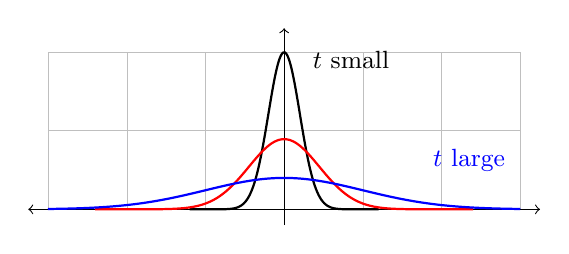
\begin{tikzpicture}
    \draw[ultra thin,color=lightgray] (-3,0) grid (3,2);
    \draw[<->] (-3.25,0) -- (3.25,0);
    \draw[->] (0,-0.2) -- (0,2.3);
    % S_d with Dt = 0.02, 0.1, 0.5 (heights 1.99,0.89,0.40)
    \draw [thick, samples=140,smooth, color=black] plot[variable=\t, domain=-1.2:1.2] ({\t},{(1/(sqrt(4*pi*0.02)))*exp(-\t*\t/(4*0.02))});
    \draw [thick, samples=100,smooth, color=red] plot[variable=\t, domain=-2.4:2.4] ({\t},{(1/(sqrt(4*pi*0.1)))*exp(-\t*\t/(4*0.1))});
    \draw [thick, samples=100,smooth, color=blue] plot[variable=\t, domain=-3:3] ({\t},{(1/(sqrt(4*pi*0.5)))*exp(-\t*\t/(4*0.5))});
    \node[color=black] at (0.85, 1.9) {\small $t$ small};
    \node[color=blue] at (2.35, 0.62) {\small $t$ large};
\end{tikzpicture}
\end{center}

\begin{example}[An Initially Gaussian Temperature]
    Suppose $\theta(x, 0) = \sqrt{\frac{a}{\pi}}\,\theta_0 e^{-ax^2}$, a Gaussian pulse of area $\theta_0$. The solution is the convolution of two Gaussians, which (completing the square in the exponent, or transforming and multiplying) is another Gaussian:
    $$
    \theta(x, t) = \theta_0\sqrt{\frac{a}{\pi(1 + 4aDt)}} \exp\left(\frac{-a x^2}{1 + 4 a D t}\right).
    $$
    The width grows like $\sqrt{t}$, the height falls correspondingly, and the area -- the total heat -- stays fixed at $\theta_0$.
\end{example}

\subsection{The Forced Diffusion Equation and Duhamel's Principle}

Now add a source term:
$$
\frac{\partial \theta}{\partial t} - D\frac{\partial^2 \theta}{\partial x^2} = f(x, t), \quad \theta(x, 0) = 0.
$$
We build the Green's function $G(x, t; \xi, \tau)$, the response to a point source in both space \emph{and} time:
$$
\frac{\partial G}{\partial t} - D \frac{\partial^2 G}{\partial x^2} = \delta(x - \xi) \delta(t - \tau), \quad G = 0 \text{ at } t = 0.
$$
Fourier transforming in $x$,
$$
\frac{\partial \tilde{G}}{\partial t} + Dk^2 \tilde{G} = e^{-ik\xi} \delta(t - \tau).
$$
Multiplying by the integrating factor $e^{Dk^2 t}$ and integrating from $0$ to $t$, the delta function fires only if $\tau < t$:
$$
\tilde{G}(k, t; \xi, \tau) = e^{-ik \xi} e^{-Dk^2 (t - \tau)} H(t - \tau).
$$
But we recognise this: apart from the causality factor $H(t - \tau)$ and the shift $e^{-ik\xi}$, it's the transform of the heat kernel with $t$ replaced by $t - \tau$. Inverting,
$$
G(x, t; \xi, \tau) = H(t - \tau)\, S_d(x - \xi, t - \tau),
$$
and the solution to the forced problem is
$$
\theta(x, t) = \int_0^{t} \int_{-\infty}^{\infty} f(\xi, \tau)\, S_d(x - \xi, t - \tau) \dd \xi \dd \tau.
$$

Look carefully at the structure of this answer. The inner integral is exactly the solution of the \emph{unforced} heat equation started at time $\tau$ from initial data $f(\cdot, \tau)$. So the forced solution is a superposition, over all past times $\tau$, of free evolutions seeded by the forcing at time $\tau$: forcing acts as a continuous stream of fresh initial conditions. This correspondence between the forced problem with homogeneous initial data and the homogeneous problem with initial data is called \vocab{Duhamel's principle}.

\subsection{The Forced Wave Equation}

The same programme for the wave equation:
$$
\frac{\partial^2 \phi}{\partial t^2} - c^2 \frac{\partial^2 \phi}{\partial x^2} = f(x, t), \quad \phi(x, 0) = \phi_t(x, 0) = 0.
$$
Transforming the Green's function equation in $x$,
$$
\frac{\partial^2 \tilde{G}}{\partial t^2} + c^2 k^2 \tilde{G} = e^{-ik\xi} \delta(t - \tau).
$$
For each $k$ this is an initial value problem for a simple harmonic oscillator kicked at $t = \tau$ -- which we solved in \S 7! The causal solution is
$$
\tilde{G} = e^{-ik \xi}\, \frac{\sin \big(kc(t - \tau)\big)}{kc}\, H(t - \tau).
$$
Inverting, with $A = x - \xi$ and $B = c(t - \tau)$, oddness kills the sine part of $e^{ikA}$ and
\begin{align*}
G &= \frac{H(t - \tau)}{\pi c} \int_0^{\infty} \frac{\cos (kA) \sin (kB)}{k} \dd k \\
&= \frac{H(t - \tau)}{2\pi c}\int_0^{\infty} \frac{\sin k(A + B) - \sin k (A - B)}{k} \dd k,
\end{align*}
and by the Dirichlet discontinuous formula each integral is $\frac{\pi}{2}\sgn(\cdot)$, giving
$$
G(x, t; \xi, \tau) = \frac{H(t - \tau)}{4c}\left[\sgn(A + B) - \sgn(A - B)\right] = \frac{1}{2c} H\big(c(t - \tau) - \abs{x - \xi}\big).
$$
The Green's function of the wave equation is a spreading `top hat' of height $1/2c$: an impulse at $(\xi, \tau)$ affects exactly those points within distance $c(t - \tau)$ -- the range of influence from the characteristics picture, reappearing from pure Fourier analysis. The solution is
$$
\phi(x, t) = \frac{1}{2c}\int_0^t \int_{x - c(t - \tau)}^{x + c(t - \tau)} f(\xi, \tau) \dd \xi \dd \tau,
$$
an integral of the forcing over the backwards light cone.

\subsection{Poisson's Equation and the Free-Space Green's Function}

Finally, the elliptic case. \vocab{Poisson's equation} is the inhomogeneous Laplace equation
$$
\nabla^2 \phi = -\rho(\vv r),
$$
say in three dimensions (in electrostatics, $\rho$ is the charge density up to constants). The delta function generalises to $\R^3$ in the obvious way: $\delta^{(3)}(\vv r - \vv r') = 0$ for $\vv r \neq \vv r'$ and $\int f(\vv r) \delta^{(3)}(\vv r - \vv r')\dd V = f(\vv r')$.

First we work on all of $\R^3$ with $\phi \to 0$ at infinity, seeking the \vocab{free-space Green's function}
$$
\nabla^2 G_{\text{FS}}(\vv r; \vv r') = \delta^{(3)}(\vv r - \vv r').
$$
Translating so $\vv r' = 0$, everything is spherically symmetric, so $G_{\text{FS}} = G(r)$. Integrate the defining equation over a ball $B_r$ of radius $r$ centred at the origin: the right side gives $1$, while the divergence theorem turns the left side into a flux,
$$
\int_{B_r} \nabla^2 G \dd V = \int_{\partial B_r} \nabla G \cdot \hat{\vv n} \dd S = 4 \pi r^2 \frac{\dd G}{\dd r}.
$$
Hence
$$
\frac{\dd G}{\dd r} = \frac{1}{4 \pi r^2} \implies G = -\frac{1}{4 \pi r} + \text{const},
$$
and decay at infinity kills the constant. Restoring the source point,
$$
G_{\text{FS}}(\vv r; \vv r') = \frac{-1}{4 \pi \abs{\vv r - \vv r'}},
$$
which is (minus) the Coulomb potential of a unit point charge. The solution of Poisson's equation in free space is therefore
$$
\phi(\vv r) = \frac{1}{4\pi} \int_{\R^3} \frac{\rho(\vv r')}{\abs{\vv r - \vv r'}} \dd V',
$$
exactly the superposition-of-point-charges formula from electrostatics.

\begin{remark}
    In two dimensions the same computation gives $G_{\text{FS}} = \frac{1}{2\pi} \log r$ -- the $\log r$ solution we discarded by regularity when separating variables in plane polars was the point-source solution all along.
\end{remark}

\subsection{Green's Identities and Boundary Value Problems}

To handle Poisson's equation on a bounded domain $D$ with boundary data, we need a few integral identities. For twice differentiable $\phi, \psi$, the divergence theorem applied to $\phi \nabla \psi$ gives \vocab{Green's first identity}
$$
\int_{\partial D} \phi \frac{\partial \psi}{\partial n} \dd S = \int_D \left(\phi \nabla^2 \psi + \nabla \phi \cdot \nabla \psi \right) \dd V,
$$
and antisymmetrising in $\phi \leftrightarrow \psi$, \vocab{Green's second identity}
$$
\int_{\partial D} \left(\phi \frac{\partial \psi}{\partial n} - \psi \frac{\partial \phi}{\partial n}\right) \dd S = \int_D \left(\phi \nabla^2 \psi - \psi \nabla^2 \phi\right) \dd V.
$$

Now take $\psi = G_{\text{FS}}(\vv r; \vv r')$ and let $\phi$ solve $\nabla^2 \phi = -\rho$. There's a subtlety: $G_{\text{FS}}$ is singular at $\vv r'$, so we excise a small ball $\mathcal{B}_\epsilon$ around $\vv r'$ and apply the second identity on $D \setminus \mathcal{B}_\epsilon$. On the small sphere $\partial \mathcal{B}_\epsilon$, we have $G_{\text{FS}} \sim -1/4\pi\epsilon$ and $\partial G_{\text{FS}}/\partial n \sim -1/4 \pi \epsilon^2$ (with the normal pointing towards $\vv r'$), so as $\epsilon \to 0$,
$$
\int_{\partial \mathcal{B}_\epsilon} \left(\phi \frac{\partial G_{\text{FS}}}{\partial n} - G_{\text{FS}} \frac{\partial \phi}{\partial n}\right) \dd S \longrightarrow -\phi(\vv r'),
$$
since the first term integrates $\phi$ against a shrinking sphere of total `weight' $-1$ and the second vanishes like $\epsilon$. The result is \vocab{Green's third identity}:
$$
\phi(\vv r') = -\int_D G_{\text{FS}}(\vv r; \vv r') \rho(\vv r) \dd V + \int_{\partial D} \left(\phi \frac{\partial G_{\text{FS}}}{\partial n} - G_{\text{FS}} \frac{\partial \phi}{\partial n}\right) \dd S.
$$
This expresses $\phi$ anywhere inside $D$ in terms of the source and \emph{both} $\phi$ and $\partial \phi/\partial n$ on the boundary. But for a Dirichlet problem we only \emph{know} $\phi$ on the boundary -- the normal derivative term is unwanted baggage.

The fix is elegant. Define the \vocab{Dirichlet Green's function} of the domain by
$$
G(\vv r; \vv r') = G_{\text{FS}}(\vv r; \vv r') + H(\vv r; \vv r'),
$$
where $H$ is harmonic in $D$ ($\nabla^2 H = 0$) and is chosen so that $G = 0$ for $\vv r \in \partial D$. Running Green's second identity with $H$ (which has no singularity) and adding it to the third identity, all the $H$ corrections combine and the $\partial \phi/\partial n$ term drops out (its coefficient $G$ vanishes on $\partial D$). With Dirichlet data $\phi = h$ on $\partial D$:
$$
\phi(\vv r') = -\int_D G(\vv r; \vv r') \rho(\vv r) \dd V + \int_{\partial D} h(\vv r) \frac{\partial G}{\partial n}(\vv r; \vv r') \dd S.
$$
The first term is the familiar Green's function solution; the second implements the inhomogeneous boundary conditions.

\subsection{The Method of Images}

Everything now rests on finding the harmonic correction $H$ -- and for symmetric domains there is a lovely trick: place fictitious \vocab{image sources} \emph{outside} the domain, positioned so that their combined potential cancels on the boundary.

\begin{example}[Laplace's Equation on a Half-Space]
    Solve $\nabla^2 \phi = 0$ in the half-space $z > 0$, with $\phi(x, y, 0) = h(x, y)$ and $\phi \to 0$ at infinity.
    For a source at $\vv r' = (x', y', z')$ with $z' > 0$, place an equal and \emph{opposite} image at the mirror point $\vv r'' = (x', y', -z')$:
    $$
    G(\vv r; \vv r') = \frac{-1}{4 \pi \abs{\vv r - \vv r'}} + \frac{1}{4 \pi \abs{\vv r - \vv r''}}.
    $$
    The image term is harmonic inside $z > 0$ (its singularity is at $z < 0$), and on the plane $z = 0$ every point is equidistant from $\vv r'$ and $\vv r''$, so $G = 0$ there: this \emph{is} the Dirichlet Green's function. Computing the normal derivative on the boundary,
    $$
    \left.\frac{\partial G}{\partial n}\right|_{z = 0} = \frac{z'}{2 \pi}\left[(x - x')^2 + (y - y')^2 + z'^2\right]^{-3/2},
    $$
    so the solution of the boundary value problem is
    $$
    \phi(x', y', z') = \frac{z'}{2\pi} \int_{-\infty}^{\infty}\int_{-\infty}^{\infty} \frac{h(x, y) \dd x \dd y}{\left[(x - x')^2 + (y - y')^2 + z'^2\right]^{3/2}}.
    $$
\end{example}

\begin{example}[Images for the Wave Equation]
    The method works for time-dependent problems too. To solve the wave equation on the half-line $x > 0$ with a fixed end $\phi(0, t) = 0$, take the free-space causal Green's function and subtract its mirror image:
    $$
    G(x, t; \xi, \tau) = \frac{1}{2c}H\big(c(t - \tau) - \abs{x - \xi}\big) - \frac{1}{2c}H\big(c(t - \tau) - \abs{x + \xi}\big),
    $$
    which vanishes at $x = 0$ for all time. (Adding instead of subtracting the image gives a free end -- a Neumann condition.) Concretely, a leftward-travelling pulse started near $\xi > 0$ meets its opposite-signed image emerging from the boundary, and the result is the familiar picture of a wave reflecting off a fixed end with inverted phase -- in agreement with the $B = -A$ limit of our reflection analysis in \S 3.
\end{example}

And with that, the toolbox is complete. It is worth stepping back to admire how the pieces interlock: separation of variables turns PDEs into Sturm--Liouville problems; completeness of eigenfunctions is the delta function's expansion; the delta function defines Green's functions; Fourier transforms construct them; and the characteristics of the equation dictate the causal structure that the Green's functions faithfully reproduce. Linearity, exploited from every possible direction.

